\documentclass[11pt,a4paper]{article}

\usepackage[T1]{fontenc}
\usepackage[utf8]{inputenc}
\usepackage[margin=2.4cm]{geometry}
\usepackage{amsmath,amssymb,amsthm,mathtools}
\usepackage{microtype}
\usepackage{graphicx}
\usepackage{booktabs}
\usepackage{array}
\usepackage{xcolor}
\usepackage{enumitem}
\usepackage{caption}
\usepackage{multicol}
\usepackage[most]{tcolorbox}
\usepackage{tikz}
\usetikzlibrary{arrows.meta,positioning,calc,fit,backgrounds,decorations.pathreplacing}
\usepackage{pgfplots}
\pgfplotsset{compat=1.18}
\usepackage{listings}
\usepackage[round,authoryear]{natbib}
\usepackage[colorlinks=true,linkcolor=tutblue!70!black,citecolor=tutblue!70!black,urlcolor=tutblue!70!black]{hyperref}
\usepackage[capitalise,noabbrev]{cleveref}

% ---------- colours (the same blue, red and grey as in the data figures) ----------
\definecolor{tutblue}{HTML}{2A78D6}
\definecolor{tutred}{HTML}{D9483B}
\definecolor{tutgrey}{HTML}{52514E}
\definecolor{tutpaper}{HTML}{F0EFEC}
\definecolor{tutgreen}{HTML}{1B8F66}

% ---------- theorem-like environments ----------
\theoremstyle{plain}
\newtheorem{proposition}{Proposition}[section]
\newtheorem{lemma}[proposition]{Lemma}
\theoremstyle{definition}
\newtheorem{definition}[proposition]{Definition}
\newtheorem{example}[proposition]{Example}
\newtheorem{exercise}{Exercise}[section]
\theoremstyle{remark}
\newtheorem{remark}[proposition]{Remark}

% ---------- boxes ----------
\newtcolorbox{intuition}{enhanced, breakable, colback=tutblue!5, colframe=tutblue, boxrule=0pt, leftrule=2.5pt,
  arc=0pt, left=8pt, right=8pt, top=5pt, bottom=5pt, before skip=9pt, after skip=9pt,
  fontupper=\small, before upper={\textbf{\textcolor{tutblue!70!black}{Intuition.}}\ }}
\newtcolorbox{caution}{enhanced, breakable, colback=tutred!5, colframe=tutred, boxrule=0pt, leftrule=2.5pt,
  arc=0pt, left=8pt, right=8pt, top=5pt, bottom=5pt, before skip=9pt, after skip=9pt,
  fontupper=\small, before upper={\textbf{\textcolor{tutred!80!black}{Caution.}}\ }}
\newtcolorbox{takeaways}{enhanced, colback=tutpaper!60, colframe=tutgrey, boxrule=0pt, leftrule=2.5pt,
  arc=0pt, left=8pt, right=8pt, top=5pt, bottom=5pt, before skip=10pt, after skip=6pt,
  fontupper=\small, before upper={\textbf{Takeaways.}\ }}

% exercises sit in the running text, so they get a frame of their own
\tcolorboxenvironment{exercise}{enhanced, breakable, colback=tutgreen!4, colframe=tutgreen, boxrule=0pt,
  leftrule=2.5pt, arc=0pt, left=8pt, right=8pt, top=4pt, bottom=4pt, before skip=9pt, after skip=9pt}
\newcommand{\extitle}[2]{#1, \textsc{#2}}
% annotated reading list at the end of a section
\newenvironment{readinglist}{\subsection*{Recommended reading}\small
  \begin{itemize}[leftmargin=1.4em, itemsep=3pt, topsep=3pt]}{\end{itemize}}

% ---------- macros ----------
\newcommand{\by}[1]{\textcolor{black!55}{\text{#1}}}   % justification of a line, set on the right
\newcommand{\R}{\mathbb{R}}
\newcommand{\E}{\mathbb{E}}
\newcommand{\LN}{\mathrm{LN}}
\newcommand{\head}{\mathrm{head}}
\newcommand{\mlp}{\mathrm{mlp}}
\newcommand{\logit}{\mathrm{logit}}
\newcommand{\relu}{\mathrm{ReLU}}
\newcommand{\clean}{\mathrm{clean}}
\newcommand{\corr}{\mathrm{corr}}
\newcommand{\one}{\mathbf{1}}
\newcommand{\Wenc}{W_{\mathrm{enc}}}
\newcommand{\Wdec}{W_{\mathrm{dec}}}
\newcommand{\benc}{b_{\mathrm{enc}}}
\newcommand{\bdec}{b_{\mathrm{dec}}}
\newcommand{\tok}[1]{\texttt{#1}}
\DeclareMathOperator{\mean}{mean}
\DeclareMathOperator{\scale}{scale}
\DeclareMathOperator{\softmax}{softmax}

% ---------- listings ----------
\lstdefinestyle{tutpython}{language=Python, basicstyle=\ttfamily\footnotesize, keywordstyle=\color{tutblue!80!black},
  commentstyle=\color{tutgrey}, stringstyle=\color{tutred!80!black}, showstringspaces=false, columns=fullflexible, basewidth=0.525em,
  keepspaces=true, frame=single, rulecolor=\color{black!25}, framesep=5pt, xleftmargin=6pt, xrightmargin=6pt,
  aboveskip=8pt, belowskip=4pt}

\captionsetup{font=small, labelfont=bf}
\setlist{itemsep=2pt, topsep=4pt}
\setlength{\parskip}{3pt plus 1pt}

\title{\textbf{Opening the Black Box}\\[4pt]
\Large A First Course in the Interpretability of Large Language Models}
\author{}
\date{November 2026}

\begin{document}
\maketitle
\vspace{-3.2em}

\begin{abstract}
\noindent
A large language model is a function with billions of learned parameters. We can read every one of them,
and still we do not know what algorithm they implement. Interpretability is the research field that tries to close
this gap. This tutorial is a first course for readers who know linear algebra, basic probability and what a neural
network is, and who have never looked inside a language model. It covers the main ideas of the field in the order
in which a practitioner meets them: the transformer written as a sum of components, methods that read activations
(attention patterns, attribution, the logit lens, probes), the linear representation and superposition hypotheses,
sparse autoencoders, causal interventions (ablation, activation patching, steering), and circuits. Every claim that
can be proved is proved in full, with each line justified. The main methods are applied to one running example, the
indirect object identification task in GPT-2 small, with numbers and figures produced by a short script that
accompanies the text. Equal space is given to the limits of each method, because the main skill in this field is
knowing what a result does not show. More than fifty exercises, derivations as well as questions for reflection,
are placed directly after the material that they use. Every section closes with an annotated list of recommended
reading from the peer-reviewed literature.
\end{abstract}

\section*{Expected learning outcomes}

After working through this tutorial and its exercises, the reader will be able to do the following.
\begin{enumerate}[leftmargin=2em, itemsep=3pt]
\item \textbf{Describe the model.} Write the computation of a transformer of the GPT type as a sequence of
additions to a residual stream, and decompose a logit into the direct contributions of all components
(\cref{sec:transformer}).
\item \textbf{Classify evidence.} Tell observational, interventional and mechanistic evidence apart, and say
which kind a given claim about a model requires (\cref{sec:intro,sec:pitfalls}).
\item \textbf{Read activations.} Use attention patterns, integrated gradients, the logit lens, direct logit
attribution and linear probes, prove the completeness of integrated gradients, and state what each of these
methods cannot show (\cref{sec:observation}).
\item \textbf{Reason about representations.} State the linear representation hypothesis and the superposition
hypothesis, prove that a high-dimensional space holds exponentially many almost orthogonal directions, and solve
a small model of superposition by hand (\cref{sec:features}).
\item \textbf{Work with sparse autoencoders.} Define a sparse autoencoder, derive the shrinkage that its sparsity
penalty causes, judge a dictionary by several criteria at once, and test whether a latent deserves its label
(\cref{sec:sae}).
\item \textbf{Intervene.} Design an activation patching experiment by choosing the two prompts, the metric and
the nodes, distinguish sufficiency from necessity and direct effects from total effects, and derive attribution
patching as a first-order approximation (\cref{sec:interventions}).
\item \textbf{Steer.} Estimate a direction from contrasting prompts, and use activation addition and directional
ablation to test whether the direction controls a behaviour (\cref{sec:lrh,sec:steering}).
\item \textbf{Explain circuits.} Define a circuit and the criteria by which it is validated, read a one-layer
attention-only model from its weights, and reconstruct the arguments behind three case studies: induction heads,
indirect object identification and modular addition (\cref{sec:circuits}).
\item \textbf{Doubt.} Recognise the common ways in which an interpretability result can mislead, and name the
control experiment that guards against each of them (\cref{sec:pitfalls}).
\item \textbf{Continue alone.} Run a patching experiment on GPT-2 small with open-source tools, and find the
peer-reviewed literature on each topic through the reading lists (\cref{sec:practice}).
\end{enumerate}

\section*{Contents}
\vspace{-0.5em}
{\small \setlength{\parskip}{0pt} \setlength{\columnsep}{22pt}
\begin{multicols}{2}
\makeatletter\@starttoc{toc}\makeatother
\end{multicols}}

\section{What does it mean to understand a language model?}
\label{sec:intro}

\subsection{The gap between knowing the weights and knowing the algorithm}

A large language model (LLM) takes a piece of text and returns a probability distribution over the next token.
Inside, it is a long but completely explicit computation: matrix products, additions, a few simple nonlinear
functions. Nothing is hidden from us. We can print any weight and record any intermediate number.

And yet we cannot say how the model works in the sense in which we can say how a sorting algorithm works. The
weights were not written by a programmer. They were found by gradient descent on a prediction loss, and the
algorithm they implement is something we have to discover after the fact. The situation resembles holding the
compiled binary of a program without its source code. Every instruction is visible, and the logic is not.

\emph{Interpretability} is the study of how to recover that logic. We use the following working definition.

\begin{definition}[Interpretability]\label{def:interp}
An \emph{interpretation} of a model is a description of its internal computation that is (i) understandable by
a human and (ii) \emph{faithful}, which means that the description correctly predicts what the model computes,
including what it computes when we intervene on its internals.
\emph{Mechanistic interpretability} is the part of the field that aims at descriptions on the level of
algorithms: which quantities the model represents, where, and through which operations they are combined.
\end{definition}

The two requirements pull in opposite directions. The full list of weights is perfectly faithful and not
understandable. A one-sentence story such as ``the model looks for the subject of the sentence'' is understandable
and may be false. The whole field lives in the tension between the two, and most of its methodological care goes
into checking condition (ii).

\subsection{Why not simply ask the model?}

A modern LLM will explain its own answers when asked. These explanations are text generated by the same model,
and nothing forces them to describe the computation that produced the answer. \citet{turpin2023language} gave a
clean demonstration. They biased multiple-choice prompts, for instance by arranging the few-shot examples so that
the correct answer was always option (A). The models then often chose (A) on the test question and wrote a
step-by-step justification of it that never mentioned the pattern that had caused the choice.

The literature separates two properties of an explanation \citep{jacovi2020towards}. An explanation is
\emph{plausible} if it convinces a human reader, and it is \emph{faithful} if it reflects the true reasoning process
of the model. Self-explanations are selected for plausibility. Interpretability research is the attempt to obtain
faithfulness, and for that we have to look inside.

\subsection{Why it matters}

We give four reasons, in decreasing order of how often they are cited.

\begin{itemize}
\item \textbf{Safety and auditing.} We would like to check properties of a model that its behaviour on a test set
cannot reveal, for example whether it pursues an objective that it does not state. \citet{marks2025auditing}
trained a model with a hidden objective and let blinded teams try to find it. Tools that read internal
activations were among the ones that helped.
\item \textbf{Debugging and control.} If we know where and how a behaviour is computed, we can change it in a
targeted way. \Cref{sec:interventions} shows how adding one vector to the activations can switch a behaviour on
or off.
\item \textbf{Science.} Neural networks generalise in ways we do not fully understand. Reading off the algorithm
that a trained network implements turns questions about generalisation into questions about concrete mechanisms.
\Cref{sec:modadd} contains an example in which a small network was reverse engineered completely.
\item \textbf{Trust.} High-stakes uses of a model call for reasons, and the reasons should be the real ones.
\end{itemize}

\subsection{Three questions and three kinds of evidence}

\begin{table}[t]
\centering\small
\begin{tabular}{@{}>{\raggedright\arraybackslash}p{0.29\textwidth}>{\raggedright\arraybackslash}p{0.37\textwidth}p{0.14\textwidth}l@{}}
\toprule
Method & What it tells us & Evidence & Where \\
\midrule
Attention patterns & from which positions a head reads & observational & \cref{sec:attention} \\
Input attribution & which input tokens the output is sensitive to & observational & \cref{sec:attribution} \\
Logit lens, direct logit attribution & when, and by which component, the answer is written & observational & \cref{sec:lens} \\
Probing & what is decodable from an activation & observational & \cref{sec:probing} \\
Sparse autoencoders & a candidate dictionary of features & observational & \cref{sec:sae} \\
Ablation, activation patching & which components the behaviour depends on & interventional & \cref{sec:interventions} \\
Steering & whether a direction controls a behaviour & interventional & \cref{sec:steering} \\
Circuit analysis & the algorithm & mechanistic & \cref{sec:circuits} \\
\bottomrule
\end{tabular}
\caption{The methods covered in this tutorial. ``Observational'' methods only record activations, and
``interventional'' methods change them. A dictionary found by a sparse autoencoder is observational evidence
until its features have been tested by interventions.}
\label{tab:map}
\end{table}

Almost every paper in the field asks one of three questions about a model and a behaviour of interest.
\begin{enumerate}[label=\textbf{Q\arabic*.}, leftmargin=3em]
\item \emph{Representation.} What information is present in the activations, and in what form?
\item \emph{Localisation.} Which parts of the model matter for the behaviour?
\item \emph{Algorithm.} What computation do these parts carry out, and why does it produce the behaviour?
\end{enumerate}
The methods differ in the kind of evidence they give, and it pays to keep the kinds apart from the first day.
\emph{Observational} methods record activations on some inputs and look for structure. They are cheap, and they
establish correlations only. \emph{Interventional} methods change an activation and measure the effect on the
output. They establish causal claims, relative to the specific intervention that was made. \emph{Mechanistic}
explanations go one step further and derive the behaviour from the weights, so that the explanation also covers
inputs that were never tried. \Cref{tab:map} places the methods of this tutorial on this map.


\subsection{The running example}
\label{sec:running}

Abstract descriptions of methods are hard to digest. We therefore apply every method to the same small task, so
that the reader can see how the different kinds of evidence fit together. The task is \emph{indirect object
identification} (IOI), introduced by \citet{wang2023interpretability}. Consider the sentence
\begin{center}
\tok{When Mary and John went to the store, John gave a drink to}
\end{center}
A fluent reader continues with \tok{Mary}. To do so, one has to notice that two names were introduced, that
\tok{John} appears a second time as the subject of the second clause, and that the remaining name is the
recipient. The name that should be predicted is called the indirect object (IO), and the repeated name is called
the subject (S).

Our model is GPT-2 small \citep{radford2019language}. It is public, it runs on a laptop, and it solves this task.
We use 12 prompts that follow the template above with six pairs of names in both orders. On all 12 prompts the
most likely next token is the correct name, with an average probability of $0.48$, against $0.014$ for the
repeated name.

\begin{caution}
All numbers and data figures about GPT-2 small in this tutorial were produced by the script
\texttt{code/gpt2\_examples.py} that accompanies the text. They are meant as illustrations on 12 prompts
from one template. They agree qualitatively with \citet{wang2023interpretability}, who studied the task on a much
larger and more varied set of prompts, and they should not be read as new findings.
\end{caution}

\subsection{How to read this tutorial}

\begin{figure}[t]
\centering
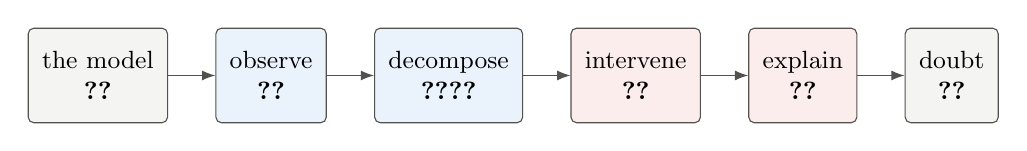
\begin{tikzpicture}[>=Latex, font=\small, node distance=6mm,
  stage/.style={draw=tutgrey, rounded corners=2pt, align=center, minimum height=12mm, inner sep=5pt, fill=#1},
  stage/.default=tutpaper!70]
\node[stage] (m) {the model\\ \cref{sec:transformer}};
\node[stage=tutblue!10, right=of m] (o) {observe\\ \cref{sec:observation}};
\node[stage=tutblue!10, right=of o] (f) {decompose\\ \cref{sec:features,sec:sae}};
\node[stage=tutred!10, right=of f] (i) {intervene\\ \cref{sec:interventions}};
\node[stage=tutred!10, right=of i] (c) {explain\\ \cref{sec:circuits}};
\node[stage, right=of c] (v) {doubt\\ \cref{sec:pitfalls}};
\foreach \a/\b in {m/o,o/f,f/i,i/c,c/v} \draw[->, tutgrey] (\a) -- (\b);
\end{tikzpicture}
\caption{Road map. Blue stages produce hypotheses from recorded activations, and red stages test them by changing
activations. The last stage collects the ways in which each of the earlier ones can mislead.}
\label{fig:roadmap}
\end{figure}

The text assumes linear algebra (vectors, matrices, inner products, projections), basic probability and the idea
of training a neural network by gradient descent. It does not assume any knowledge of transformers, which
\cref{sec:transformer} introduces from scratch. The order of the sections follows \cref{fig:roadmap}.

Three kinds of boxes mark material with a special role. An \emph{Intuition} box gives an informal picture of a
formal statement. A \emph{Caution} box states a limit of a method or a common misreading. A \emph{Takeaways} box
closes each section. Symbols are defined at the place where they are first used. Proofs are written as chains of
equalities in which the reason for each line is printed in grey on the right. Each section ends with a few
exercises, and \cref{app:solutions} contains solutions. A glossary of the technical terms is in
\cref{app:glossary}. Finally, \cref{sec:practice} lists software, first projects and further reading.

\section{The object of study: a transformer in equations}
\label{sec:transformer}

Before we can interpret a model we need a precise description of what it computes. This section defines a
decoder-only transformer of the GPT-2 type \citep{vaswani2017attention,radford2019language} and extracts the
structural facts on which the methods of the later sections rest. The presentation follows the ``residual
stream'' view of \citet{elhage2021mathematical}.

\subsection{From text to a prediction}

A \emph{tokenizer} cuts the input text into pieces called \emph{tokens}, which are words or fragments of words,
and replaces each piece by its index in a fixed vocabulary of size $V$. The input of the model is therefore a
sequence of indices $t_1,\dots,t_n$ with $t_i\in\{1,\dots,V\}$. For every position $i$ the model returns a vector
of $V$ real numbers called \emph{logits}. We write $\logit_i(t)$ for the logit of token $t$ at position $i$. The
predicted probability that the next token $t_{i+1}$ equals $t$ is the softmax of the logits,
\begin{equation}\label{eq:softmax}
\Pr(t_{i+1}=t \mid t_1,\dots,t_i) \;=\; \frac{\exp(\logit_i(t))}{\sum_{t'=1}^{V}\exp(\logit_i(t'))} .
\end{equation}
Training adjusts the weights so as to minimise the average of $-\log\Pr(t_{i+1}\mid t_1,\dots,t_i)$ over a large
corpus of text. This quantity is called the cross-entropy loss, and it is small when the true next token receives a
high probability.

\begin{exercise}[\extitle{Softmax sees only differences}{derivation}]\label{ex:softmax}
(a) Show that adding the same number to all logits at position $i$ does not change the probabilities
\eqref{eq:softmax}. (b) Show that the ratio of the probabilities of two tokens $t$ and $t'$ equals
$\exp(\logit_i(t)-\logit_i(t'))$. (c) Let $t^\star$ be the true next token. Show that the derivative of the loss
$-\log\Pr(t_{i+1}=t^\star\mid t_1,\dots,t_i)$ with respect to $\logit_i(t)$ equals
$\Pr(t_{i+1}=t\mid t_1,\dots,t_i)-1$ if $t=t^\star$ and $\Pr(t_{i+1}=t\mid t_1,\dots,t_i)$ if $t\ne t^\star$.
(d) What do (a) to (c) suggest about the right way to measure how well a model separates two candidate tokens?
\end{exercise}

\subsection{The residual stream}

The model keeps, for every position $i$, a vector in $\R^d$ that is updated layer by layer. This vector is called
the \emph{residual stream} at position $i$. We write $x_i^{(\ell)}\in\R^d$ for its value at the input of layer
$\ell$, where the layers are numbered $\ell=0,\dots,L-1$, and $x_i^{(L)}$ for its final value.
\Cref{fig:residual} shows the flow of the computation.

\paragraph{Embedding.} The stream starts as the sum of a vector for the token and a vector for the position,
\begin{equation}\label{eq:embed}
x_i^{(0)} \;=\; W_E[t_i] + W_{\mathrm{pos}}[i],
\end{equation}
where $W_E[t]\in\R^d$ denotes the column of the embedding matrix $W_E\in\R^{d\times V}$ that belongs to token $t$,
and $W_{\mathrm{pos}}[i]\in\R^d$ is a learned vector for position $i$.

\paragraph{Layer normalisation.} Every component reads the stream through the map
\begin{equation}\label{eq:ln}
\LN(x) \;=\; \frac{x-\mean(x)\,\one}{\scale(x)},\qquad
\mean(x)=\frac1d\,\one^\top x,\qquad
\scale(x)=\frac{1}{\sqrt d}\,\big\|x-\mean(x)\,\one\big\|,
\end{equation}
where $\one\in\R^d$ is the vector of ones and $\|\cdot\|$ is the Euclidean norm. $\LN$ subtracts the average coordinate and rescales the result to a
fixed length. The original definition also multiplies by a learned vector and adds another one. Since $\LN$ is
always followed by a linear map, these two learned vectors can be absorbed into that map and its bias, and we do
so throughout.

\paragraph{Attention heads.} Layer $\ell$ contains $H$ attention heads, numbered $h=0,\dots,H-1$. A head is the
only kind of component that moves information between positions. Head $h$ of layer $\ell$ has four weight matrices
$W_Q,W_K,W_V\in\R^{d_{\mathrm{head}}\times d}$ and $W_O\in\R^{d\times d_{\mathrm{head}}}$ (each head has its own,
and we suppress the indices $\ell,h$ on them). The width $d_{\mathrm{head}}$ of a head is much smaller than
$d$. They enter only through the two products
\begin{equation}\label{eq:qkov}
W_{QK} \;=\; W_Q^\top W_K\in\R^{d\times d},\qquad W_{OV} \;=\; W_O W_V\in\R^{d\times d}.
\end{equation}
For a position $i$ and every earlier or equal position $j\le i$, the head computes a score, turns the scores into
weights by a softmax over $j$, and outputs a weighted sum:
\begin{align}
A^{\ell,h}_{ij} &\;=\; \frac{\exp\!\big(\LN(x_i^{(\ell)})^\top W_{QK}\,\LN(x_j^{(\ell)})/\sqrt{d_{\mathrm{head}}}\big)}
{\sum_{j'\le i}\exp\!\big(\LN(x_i^{(\ell)})^\top W_{QK}\,\LN(x_{j'}^{(\ell)})/\sqrt{d_{\mathrm{head}}}\big)},
\label{eq:pattern}\\
\head_i^{\ell,h} &\;=\; \sum_{j\le i}A^{\ell,h}_{ij}\;W_{OV}\,\LN(x_j^{(\ell)}) \;\in\R^d. \label{eq:headout}
\end{align}
The numbers $A^{\ell,h}_{ij}\ge 0$ sum to one over $j$ and are called the \emph{attention pattern} of the head.
We call $i$ the \emph{destination} and $j$ the \emph{source}. In the usual terminology,
$W_Q\LN(x_i^{(\ell)})$ is the \emph{query} of the destination, $W_K\LN(x_j^{(\ell)})$ is the \emph{key} of the source
and $W_V\LN(x_j^{(\ell)})$ is its \emph{value}. The score is the inner product of query and key, so a source
receives a large weight if its key matches what the destination asks for. The two products in \eqref{eq:qkov} have separate
jobs. $W_{QK}$ decides \emph{from where} position $i$ reads, and $W_{OV}$ decides \emph{what} is written to
position $i$ once a source has been chosen. The restriction $j\le i$ ensures that a position never sees later
tokens.

\paragraph{MLP.} After the heads, layer $\ell$ applies a two-layer perceptron to every position separately. With
$\tilde x_i^{(\ell)}$ denoting the stream after the heads of layer $\ell$,
\begin{equation}\label{eq:mlp}
\mlp_i^{\ell} \;=\; W_{\mathrm{out}}\,\mathrm{GELU}\big(W_{\mathrm{in}}\,\LN(\tilde x_i^{(\ell)})+b_{\mathrm{in}}\big)+b_{\mathrm{out}} \;\in\R^d,
\end{equation}
with weight matrices $W_{\mathrm{in}}$, $W_{\mathrm{out}}$ and bias vectors $b_{\mathrm{in}}$, $b_{\mathrm{out}}$ that
belong to the layer. Here $\mathrm{GELU}$ is a smooth variant of $\max(0,\cdot)$ applied to each coordinate. The coordinates of the
vector inside $\mathrm{GELU}$ are the \emph{neurons} of the layer.

\paragraph{Update rule and output.} Both kinds of components \emph{add} their output to the stream,
\begin{equation}\label{eq:update}
\tilde x_i^{(\ell)} \;=\; x_i^{(\ell)}+\sum_{h=0}^{H-1}\head_i^{\ell,h},\qquad
x_i^{(\ell+1)} \;=\; \tilde x_i^{(\ell)}+\mlp_i^{\ell},\qquad \ell=0,\dots,L-1 .
\end{equation}
The logits are a linear function of the normalised final stream. With $W_U[t]\in\R^d$ denoting the row of the
unembedding matrix $W_U\in\R^{V\times d}$ that belongs to token $t$, written as a column vector,
\begin{equation}\label{eq:unembed}
\logit_i(t) \;=\; W_U[t]^\top\,\LN\big(x_i^{(L)}\big).
\end{equation}
Two kinds of bias terms are omitted from these formulas. The linear maps inside a head have bias vectors, and
absorbing the learned shift of the final $\LN$ into the unembedding leaves a constant $b_U[t]$ that is added to the
logit of token $t$. All statements below stay true with them, if the output bias of each attention layer is counted
as one more component and $b_U[t]$ as one more summand of $\logit_i(t)$.

\begin{figure}[t]
\centering
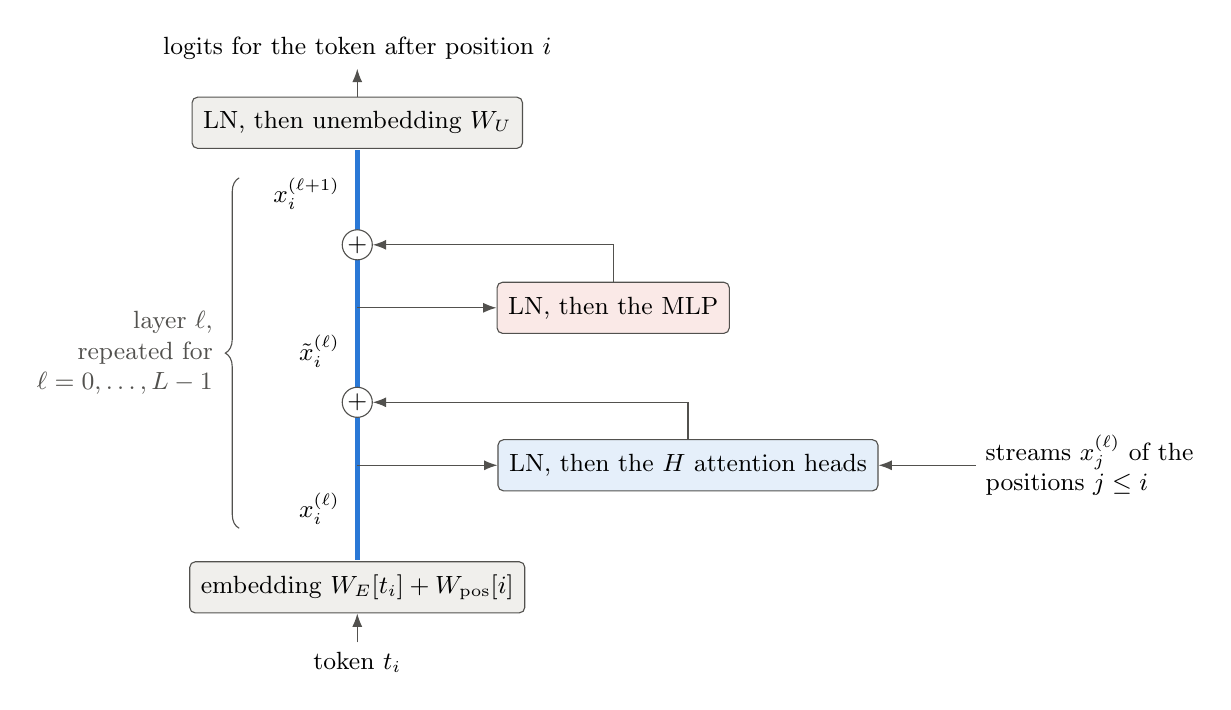
\begin{tikzpicture}[>=Latex, font=\small,
  box/.style={draw=tutgrey, rounded corners=2pt, minimum height=6.5mm, inner sep=4pt, fill=#1},
  box/.default=white, add/.style={circle, draw=tutgrey, inner sep=0.5pt, fill=white}]
\draw[line width=1.8pt, tutblue] (0,0.35) -- (0,5.55);
\node[box=tutpaper] (emb) at (0,0) {embedding $W_E[t_i]+W_{\mathrm{pos}}[i]$};
\node (tok) at (0,-0.95) {token $t_i$};
\draw[->, tutgrey] (tok) -- (emb);
\node[add] (p1) at (0,2.35) {$+$};
\node[add] (p2) at (0,4.35) {$+$};
\node[box=tutblue!12] (att) at (4.2,1.55) {$\LN$, then the $H$ attention heads};
\node[box=tutred!12] (mlp) at (3.25,3.55) {$\LN$, then the MLP};
\draw[->, tutgrey] (0,1.55) -- (att.west);
\draw[->, tutgrey] (att.north) |- (p1);
\draw[->, tutgrey] (0,3.55) -- (mlp.west);
\draw[->, tutgrey] (mlp.north) |- (p2);
\node[align=left] (others) at (9.3,1.55) {streams $x_j^{(\ell)}$ of the\\ positions $j\le i$};
\draw[->, tutgrey] (others.west) -- (att.east);
\node[box=tutpaper] (un) at (0,5.9) {$\LN$, then unembedding $W_U$};
\node (out) at (0,6.85) {logits for the token after position $i$};
\draw[->, tutgrey] (un) -- (out);
\node[left] at (-0.1,1.0) {$x_i^{(\ell)}$};
\node[left] at (-0.1,3.0) {$\tilde x_i^{(\ell)}$};
\node[left] at (-0.1,5.0) {$x_i^{(\ell+1)}$};
\draw[decorate, decoration={brace, amplitude=5pt}, tutgrey] (-1.5,0.75) -- (-1.5,5.2)
  node[midway, left=6pt, align=right] {layer $\ell$,\\ repeated for\\ $\ell=0,\dots,L-1$};
\end{tikzpicture}
\caption{The residual stream at one position $i$ (thick blue line). Each component reads the stream through
$\LN$ and adds its output back. Only the attention heads see the streams of other positions.}
\label{fig:residual}
\end{figure}

\paragraph{Sizes.} GPT-2 small has $L=12$ layers, $H=12$ heads per layer, stream width $d=768$,
$d_{\mathrm{head}}=64$, $3072$ neurons per MLP, a vocabulary of $V=50257$ tokens and about $124$ million
parameters. It is customary to name a head by layer and index, so that ``head 9.6'' is head $h=6$ of layer
$\ell=9$. Current large models have the same architecture up to details and are larger by two to three orders of
magnitude.

\begin{exercise}[\extitle{Attention by hand}{derivation}]\label{ex:byhand}
Consider one head with $d=2$ and $d_{\mathrm{head}}=1$ in a model without $\LN$ and without biases. Its weights are
$W_Q=(0\ \ 2)$, $W_K=(1\ \ 0)$, $W_V=(1\ \ 0)$ and $W_O=(0\ \ 1)^\top$. The stream at the input of the layer is
$x_1^{(\ell)}=(1,0)^\top$ at position $1$ and $x_2^{(\ell)}=(0,1)^\top$ at position $2$. (a) Compute $W_{QK}$ and
$W_{OV}$. (b) Compute the attention pattern and the output of the head at the destination $i=2$. (c) Do the same
at the destination $i=1$. (d) The attention weights of a destination always sum to one, so a head cannot decide
to read from nowhere. How can a model still arrange that a head writes almost nothing at some destinations?
\end{exercise}

\begin{exercise}[\extitle{Counting parameters}{derivation}]\label{ex:params}
Count the weights of one attention head of GPT-2 small, without biases. Using the total of $124$ million
parameters, which fraction of the model is taken by the token embedding matrix $W_E$?
\end{exercise}

\begin{exercise}[\extitle{What one head can write}{derivation}]\label{ex:rank}
(a) Show that $W_{OV}$ has rank at most $d_{\mathrm{head}}$. What does this say about the set of vectors that a
single head of GPT-2 small can write to the stream? (b) In GPT-2 small, $d_{\mathrm{head}}=d/H$. What is the
largest possible dimension of the space to which the $H$ heads of one layer can write together?
\end{exercise}

\subsection{Four structural facts}
\label{sec:facts}

The following facts are immediate from the definitions, and each of them is the basis of a family of methods.

\begin{proposition}[The final stream is a sum of component outputs]\label{prop:sum}
For every position $i$,
\begin{equation}\label{eq:sum}
x_i^{(L)} \;=\; W_E[t_i]+W_{\mathrm{pos}}[i]+\sum_{\ell=0}^{L-1}\Big(\sum_{h=0}^{H-1}\head_i^{\ell,h}+\mlp_i^{\ell}\Big).
\end{equation}
\end{proposition}
\begin{proof}
We write the final stream as a telescoping sum over the layers.
\begin{align*}
x_i^{(L)} &= x_i^{(0)}+\sum_{\ell=0}^{L-1}\big(x_i^{(\ell+1)}-x_i^{(\ell)}\big) && \by{telescoping sum}\\
&= x_i^{(0)}+\sum_{\ell=0}^{L-1}\Big(\sum_{h=0}^{H-1}\head_i^{\ell,h}+\mlp_i^{\ell}\Big) && \by{by \eqref{eq:update}}\\
&= W_E[t_i]+W_{\mathrm{pos}}[i]+\sum_{\ell=0}^{L-1}\Big(\sum_{h=0}^{H-1}\head_i^{\ell,h}+\mlp_i^{\ell}\Big). && \by{by \eqref{eq:embed}}\qedhere
\end{align*}
\end{proof}

\begin{proposition}[Each logit is a sum over components, given the final scale]\label{prop:dla}
Let $\mathcal G_i$ be the set of the $2+L(H+1)$ vectors on the right-hand side of \eqref{eq:sum}. We call them
the \emph{components} at position $i$. Then for every token $t$,
\begin{equation}\label{eq:dla}
\logit_i(t) \;=\; \sum_{g\in\mathcal G_i}\frac{W_U[t]^\top\big(g-\mean(g)\,\one\big)}{\scale\big(x_i^{(L)}\big)} .
\end{equation}
\end{proposition}
\begin{proof}
We insert the definition of $\LN$ and the sum of \cref{prop:sum} into the read-out.
\begin{align*}
\logit_i(t) &= W_U[t]^\top\,\LN\big(x_i^{(L)}\big) && \by{by \eqref{eq:unembed}}\\
&= \frac{W_U[t]^\top\big(x_i^{(L)}-\mean(x_i^{(L)})\,\one\big)}{\scale(x_i^{(L)})} && \by{by \eqref{eq:ln}}\\
&= \frac{W_U[t]^\top\big(\sum_{g\in\mathcal G_i}g-\mean\big(\sum_{g\in\mathcal G_i}g\big)\,\one\big)}{\scale(x_i^{(L)})} && \by{by \cref{prop:sum}}\\
&= \sum_{g\in\mathcal G_i}\frac{W_U[t]^\top\big(g-\mean(g)\,\one\big)}{\scale(x_i^{(L)})}. && \by{since $\mean$ is linear}\qedhere
\end{align*}
\end{proof}

The summand of a component $g$ in \eqref{eq:dla} is called its \emph{direct logit attribution}. We use it in
\cref{sec:lens}. Two more facts need no proof.

\begin{itemize}
\item \textbf{Information moves between positions only through attention.} By \eqref{eq:mlp}, the output of an
MLP at position $i$ depends on the stream at position $i$ alone, and the same holds for $\LN$ and for the
unembedding. If the final position ``knows'' something about an earlier token, some attention head has carried
it there.
\item \textbf{The coordinates of the stream have no special meaning.} Every component reads the stream through
a linear map after $\LN$ and writes to it through a linear map. Let $\Omega$ be an orthogonal matrix with $\Omega\one=\one$.
Then $\LN(\Omega x)=\Omega\,\LN(x)$. If we replace the stream by $\Omega x$, multiply every reading matrix by
$\Omega^\top$ from the right and every writing matrix by $\Omega$ from the left, the model computes the same
function. Hence nothing singles out coordinate number
$17$ of the stream. The MLP neurons are different, because $\mathrm{GELU}$ acts on each coordinate separately.
We say that the neurons form a \emph{privileged basis} and that the residual stream has none.
\end{itemize}

\begin{intuition}
Think of the residual stream as a shared whiteboard with $d$ dimensions of space. Each head and each MLP reads
what is on the board, computes something, and adds its result to the board. The final answer is read off the
board by one linear map. \Cref{prop:sum,prop:dla} say that we can account for the final answer contribution by
contribution. The last fact says that the board has no natural grid: the meaningful ``places'' on it are
directions that we have to find.
\end{intuition}

\begin{exercise}[\extitle{A direction that nobody reads}{derivation}]\label{ex:ones}
Let $s\in\R$. Show that $\LN(x+s\,\one)=\LN(x)$. Conclude that replacing the stream $x_i^{(\ell)}$ by
$x_i^{(\ell)}+s\,\one$ at any single layer and position does not change any logit.
\end{exercise}

\begin{exercise}[\extitle{Rotating the stream}{derivation}]\label{ex:rotation}
(a) Prove the claim made above that $\LN(\Omega x)=\Omega\,\LN(x)$ for every orthogonal matrix $\Omega$ with
$\Omega\one=\one$. (b) Show by an example with $d=2$ that the claim fails for a general orthogonal matrix.
(c) A colleague plots coordinate number $17$ of the residual stream over many prompts and finds that it is large
on texts about sports. Use the last fact of this subsection to explain why this observation says little about
how the model represents sports.
\end{exercise}

\subsection{The running example in this notation}
\label{sec:metric}

In the IOI task of \cref{sec:running} we look at the last position $n$ and compare two tokens, the indirect object
(the correct name) and the subject (the repeated name). Our measure of performance is the \emph{logit difference}
\begin{equation}\label{eq:ld}
\logit_n(\mathrm{IO})-\logit_n(\mathrm{S}) \;=\; \big(W_U[\mathrm{IO}]-W_U[\mathrm{S}]\big)^\top\LN\big(x_n^{(L)}\big).
\end{equation}
By \eqref{eq:softmax}, the ratio of the two predicted probabilities equals the exponential of this difference.
On our 12 prompts the logit difference of GPT-2 small is $3.70$ on average and lies between $2.06$ and $5.53$.
A logit difference of $3.70$ on a prompt means that the model judges the correct name about
$e^{3.70}\approx 40$ times as likely as the repeated one on that prompt.

We prefer the logit difference to the probability of the correct name for two reasons. It is a linear function of
$\LN(x_n^{(L)})$, so \cref{prop:dla} applies to it term by term. And it removes everything that the two names have
in common. A component that only says ``the next token is a name'' raises both logits equally and cancels in
\eqref{eq:ld}.

\begin{exercise}[\extitle{What the logit difference hides}{concept}]\label{ex:metric}
Suppose that some head raises the logits of all first names by the same amount at the last position of every IOI
prompt. (a) What is its contribution to the logit difference \eqref{eq:ld}? (b) Is this head irrelevant for the
task? (c) Propose a metric under which its contribution becomes visible.
\end{exercise}

\subsection{Why the problem is hard}

Three properties of the object make interpretation difficult, and each later section responds to one of them.
The first is \emph{size}. GPT-2 small already has $144$ heads and $36{,}864$ MLP neurons, and each of them acts
at every position. The second is that information is \emph{distributed}. By the last fact of \cref{sec:facts},
a concept need not sit in one coordinate or one neuron (\cref{sec:features,sec:sae}). The third is
\emph{nonlinearity}. The attention pattern \eqref{eq:pattern}, the $\mathrm{GELU}$ and the scale in $\LN$ make
the effect of a component depend on what all the others are doing, which is why we will need interventions
(\cref{sec:interventions}) and cannot stop at decompositions.

\begin{takeaways}
A transformer keeps one vector per position, the residual stream, and every component adds to it. The final
stream is a sum of component outputs, and each logit is a sum of per-component terms once the final scale is
fixed. Attention heads are the only route between positions. The stream has no privileged coordinates, and the
MLP neurons do.
\end{takeaways}

\begin{readinglist}
\item \citet{vaswani2017attention}, \emph{NeurIPS}. The original description of the architecture. It predates the
residual-stream view, and comparing the two presentations is instructive.
\item \citet{weiss2021thinking}, \emph{ICML}. Defines a small programming language whose operations correspond to
attention and to MLP layers. Writing a task in this language shows how many layers and heads a transformer needs
for it.
\item \citet{geva2021transformer}, \emph{EMNLP}, and \citet{geva2022transformer}, \emph{EMNLP}. Two studies of the
MLP layers. The first reads their input weights as patterns that are detected and their output weights as tokens
that are promoted. The second describes the output of an MLP as a sum of updates to the stream, read through the
unembedding.
\item \citet{dar2023analyzing}, \emph{ACL}. Interprets the weights of a transformer directly, by expressing them
in the space of token embeddings, without running the model on any input.
\item \citet{lindner2023tracr}, \emph{NeurIPS}. A compiler that turns a known algorithm into the weights of a
transformer. The resulting models have a known ground truth, on which interpretability methods can be tested.
\item \citet{csordas2025language}, \emph{NeurIPS}. Uses the additive structure of the residual stream to ask how
much each layer of current large models contributes, and finds that the later layers contribute much less than
the earlier ones.
\end{readinglist}

\section{Reading activations: observational methods}
\label{sec:observation}

The cheapest thing we can do with a model is to run it on some inputs and look at the numbers it produces
along the way. This section covers four families of methods of this kind. None of them changes an activation.
All of them are best understood as generators of hypotheses, which \cref{sec:interventions} will then test.

\subsection{Attention patterns}
\label{sec:attention}

The attention pattern $A^{\ell,h}_{ij}$ of \eqref{eq:pattern} is the most accessible quantity inside a
transformer, since it directly answers the question from which positions $j$ a head reads when it writes to
position $i$. In the running example we look at the last position $i=n$, where the name has to be predicted.
Averaged over our 12 prompts, head 9.9 puts a weight of $0.79$ on the position of the indirect object, $0.03$ on
the first occurrence of the subject and $0.04$ on the second. Heads 9.6 and 10.0 show the same preference with
weights $0.59$ and $0.31$ on the indirect object. This suggests a hypothesis: these heads fetch the correct name
and write it into the last position.

Now consider head 10.7. Its pattern looks the same, with a weight of $0.82$ on the indirect object. We will see
in \cref{sec:lens} that this head \emph{lowers} the logit of the correct name. The pattern could not have told
us.

\begin{caution}
An attention pattern shows \emph{from where} a head reads. It does not show \emph{what} the head writes, which is
decided by $W_{OV}$ in \eqref{eq:headout}. Three further limits apply. First, the stream at a source position
$j$ in a late layer no longer describes token $t_j$ alone, because earlier heads have moved other information
there. Second, a large weight on a source whose value vector $W_{OV}\LN(x_j^{(\ell)})$ is small has little effect.
Third, on classification tasks \citet{jain2019attention} found that attention weights are often uncorrelated with
gradient-based importance measures, and that very different attention distributions can produce the same
prediction. \citet{wiegreffe2019attention} discuss in which sense attention can still serve as an explanation.
\end{caution}

\subsection{Input attribution}
\label{sec:attribution}

Input attribution asks which input tokens a given output depends on. Let $F$ be a scalar output of the model,
for us the logit difference \eqref{eq:ld}, regarded as a function of the token embeddings
$z=(z_1,\dots,z_n)$ with $z_i=W_E[t_i]\in\R^d$. The simplest attribution to token $i$ is the gradient
$\nabla_{z_i}F(z)$ or its norm \citep{simonyan2014deep}. The gradient measures the effect of an infinitesimal
change of $z_i$. A popular variant, \emph{gradient times input}, takes $z_i^\top\nabla_{z_i}F(z)$ as the
contribution of token $i$. This would be exact if $F$ were linear without a constant term, and in general it
is a first-order guess.

\emph{Integrated gradients} \citep{sundararajan2017axiomatic} repairs the main defect of this guess. We choose
a \emph{baseline} input $\bar z$ that stands for ``no information'' and averages the gradient along the straight
line from $\bar z$ to $z$:
\begin{equation}\label{eq:ig}
\mathrm{IG}_i(z) \;=\; (z_i-\bar z_i)^\top\int_0^1\nabla_{z_i}F\big(\bar z+u\,(z-\bar z)\big)\,du .
\end{equation}
As $u$ runs from $0$ to $1$, the input is faded in from the baseline to the real prompt, and the integral records
how strongly the output reacts to token $i$ along the way.

\begin{proposition}[Completeness of integrated gradients]\label{prop:ig}
Let $F$ be continuously differentiable on the segment between $\bar z$ and $z$. Then the attributions
\eqref{eq:ig} add up to the change of the output,
\[
\sum_{i=1}^{n}\mathrm{IG}_i(z) \;=\; F(z)-F(\bar z).
\]
\end{proposition}
\begin{proof}
We differentiate $F$ along the segment from $\bar z$ to $z$.
\begin{align*}
F(z)-F(\bar z) &= \int_0^1\frac{d}{du}F\big(\bar z+u\,(z-\bar z)\big)\,du && \by{fundamental theorem of calculus}\\
&= \int_0^1\sum_{i=1}^{n}(z_i-\bar z_i)^\top\nabla_{z_i}F\big(\bar z+u\,(z-\bar z)\big)\,du && \by{chain rule}\\
&= \sum_{i=1}^{n}(z_i-\bar z_i)^\top\int_0^1\nabla_{z_i}F\big(\bar z+u\,(z-\bar z)\big)\,du && \by{linearity of the integral}\\
&= \sum_{i=1}^{n}\mathrm{IG}_i(z). && \by{by \eqref{eq:ig}}\qedhere
\end{align*}
\end{proof}
The assumption holds for GPT-2, whose building blocks (the $\mathrm{GELU}$, the softmax, and $\LN$ away from
$\scale(x)=0$) are smooth.

\begin{table}[ht]
\centering\footnotesize
\setlength{\tabcolsep}{3.2pt}
\begin{tabular}{@{}l*{15}{r}@{}}
\toprule
 & \tok{BOS} & \tok{When} & IO & \tok{and} & S1 & \tok{went} & \tok{to} & \tok{the} & \tok{store} & \tok{,} & S2 & \tok{gave} & \tok{a} & \tok{drink} & \tok{to}\\
\midrule
IG & $1.59$ & $-0.63$ & $2.11$ & $0.43$ & $-1.96$ & $1.20$ & $0.46$ & $0.50$ & $0.38$ & $0.53$ & $-1.15$ & $0.62$ & $-0.16$ & $-0.94$ & $0.74$\\
G$\times$I & $0.62$ & $-0.24$ & $-1.53$ & $-0.35$ & $0.23$ & $-0.15$ & $-0.01$ & $-0.01$ & $-0.18$ & $0.06$ & $-0.94$ & $-0.38$ & $-0.02$ & $0.60$ & $-0.43$\\
\bottomrule
\end{tabular}
\caption{Attribution of the logit difference of GPT-2 small to the input tokens, averaged over 12 prompts. IG
denotes integrated gradients and G$\times$I gradient times input. IO is
the indirect object, S1 and S2 are the two occurrences of the subject, and \tok{BOS} is the start token that
the tokenizer prepends.}
\label{tab:ig}
\end{table}

\paragraph{The running example.} \Cref{tab:ig} shows both attributions for the logit difference, averaged over
our 12 prompts. The baseline $\bar z$ sets all token embeddings to zero and keeps the positional embeddings, and
the integral in \eqref{eq:ig} is approximated by a midpoint sum with 64 points. The integrated gradients add up to
$3.706$, while $F(z)-F(\bar z)=3.703$, so \cref{prop:ig} holds up to the discretisation error. Gradient times
input adds up to $-2.75$, which has the wrong sign. It is not a decomposition of anything.


The integrated gradients give the largest positive value to the indirect object and negative values to both
occurrences of the subject, which is sensible. But the start token and the word \tok{went} also receive more
than one logit each, although they are the same in every prompt and say nothing about which name is correct.
The reason is the baseline. Integrated gradients explain the difference between the input and the baseline,
and an all-zero input differs from a sentence in every token.

\begin{caution}
Input attribution answers the question ``which input features, relative to which baseline''. The baseline is a
modelling choice, and unusual baselines take the model far from the inputs it was trained on. Attribution maps
can also look convincing for reasons that have nothing to do with the model. \citet{adebayo2018sanity} showed
that some saliency methods for image classifiers produce nearly the same picture after the weights of the
network have been replaced by random numbers. Finally, even a perfect attribution says which inputs matter and
is silent on how they are processed. Methods such as LIME \citep{ribeiro2016should} and SHAP
\citep{lundberg2017unified} share this scope. They treat the model as a black box and fit a simple surrogate to
its input-output behaviour.
\end{caution}

\subsection{The logit lens and direct logit attribution}
\label{sec:lens}

The two methods of this subsection exploit the additive structure of \cref{sec:facts}.

\paragraph{Logit lens.} By \eqref{eq:unembed} the model reads its prediction from the final stream $x_i^{(L)}$.
Since all streams $x_i^{(\ell)}$ live in the same space, nothing stops us from applying the same read-out to an
intermediate one \citep{nostalgebraist2020logit}:
\begin{equation}\label{eq:lens}
\text{lens logit of token $t$ after $\ell$ layers} \;=\; W_U[t]^\top\,\LN\big(x_i^{(\ell)}\big),\qquad \ell=0,\dots,L .
\end{equation}
This shows what the model would predict if it had to stop after $\ell$ layers. For example, $\ell=10$ means
that the layers $0$ to $9$ have been applied. For example, $\ell=10$ means that
the layers $0$ to $9$ have been applied. \Cref{fig:lens} shows the result
for the running example. Up to $\ell=7$ the lens logit difference stays within half a logit of zero. It becomes
positive at $\ell=8$ and jumps at $\ell=10$, which is after layer 9 has been applied. On the first prompt, the most likely
token under the lens is \tok{drink} at $\ell=5$, \tok{the} at $\ell=8$, \tok{them} at $\ell=9$ and \tok{Mary}
from $\ell=10$ on. So the decision between the two names is written into the last position mainly by layer 9,
with a small start in layers 7 and 8.

The figure has a second message. After 10 layers the lens gives the correct name a probability of $0.998$, and
the complete model gives it only $0.48$. Layers 10 and 11 make the model \emph{less} confident. We will meet the
components that do this in a moment.

\begin{figure}[t]
\centering
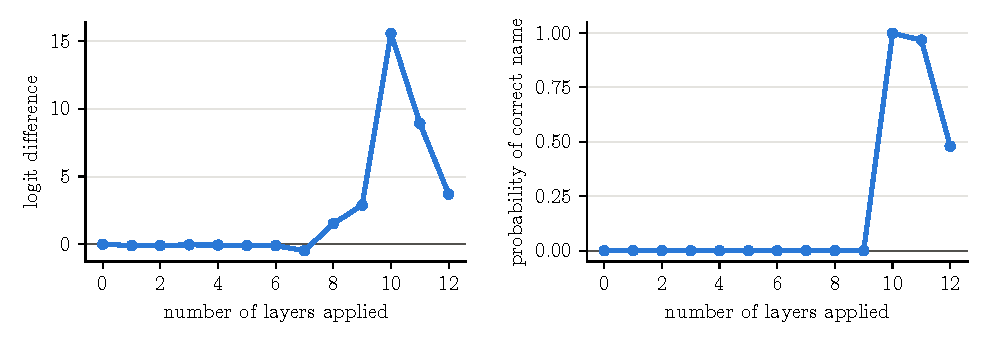
\includegraphics[width=0.82\textwidth]{figures/fig_logit_lens.pdf}
\caption{Logit lens on the IOI task in GPT-2 small, at the last position, averaged over 12 prompts. Left: lens
logit difference between the correct and the repeated name. Right: lens probability of the correct name. The
horizontal axis is the number $\ell$ of layers that have been applied, so $\ell=12$ is the real output.}
\label{fig:lens}
\end{figure}

\begin{caution}
The lens assumes that intermediate layers already use the output basis $W_U$. This is roughly true in late
layers and often false in early ones. The \emph{tuned lens} of \citet{belrose2023eliciting} relaxes the
assumption by training, for each layer, an affine map that is applied before the read-out. Magnitudes also need
care: $\LN$ in \eqref{eq:lens} rescales each intermediate stream by its own scale, so the height of the peak at
$\ell=10$ in \cref{fig:lens} is not on the scale of the final logits. Which layer makes the difference appear
is the robust part of the picture.
\end{caution}

\paragraph{Direct logit attribution.} The lens tells us \emph{when} the answer appears. \Cref{prop:dla} tells us
\emph{which component} wrote it. Applying \eqref{eq:dla} to the two tokens of \eqref{eq:ld} and subtracting gives
\begin{equation}\label{eq:dla-ld}
\logit_n(\mathrm{IO})-\logit_n(\mathrm{S}) \;=\; \sum_{g\in\mathcal G_n}
\frac{\big(W_U[\mathrm{IO}]-W_U[\mathrm{S}]\big)^\top\big(g-\mean(g)\,\one\big)}{\scale\big(x_n^{(L)}\big)} .
\end{equation}
Each summand is the \emph{direct logit attribution} (DLA) of one component: the amount by which this component,
through its own addition to the stream, moves the logit difference.

We computed all terms of \eqref{eq:dla-ld} for the running example. The terms add up to $3.7031$, and the logit
difference measured at the output is $3.7031$, as the proposition demands. The 144 heads together contribute
$3.45$, the 12 MLPs $0.25$, and the embeddings and bias terms less than $0.01$. \Cref{fig:dla} shows the heads.
Almost all of them contribute nothing. Four heads write clearly in favour of the correct name: 9.9
($+3.57$), 9.6 ($+1.10$), 10.6 ($+0.61$) and 10.0 ($+0.59$). Three of them are the heads whose attention patterns
we inspected in \cref{sec:attention}. Two heads write \emph{against} it: 10.7 ($-2.52$) and 11.10 ($-1.05$). They
sit in layers 10 and 11, which explains the drop after $\ell=10$ in \cref{fig:lens}.
\citet{wang2023interpretability} call 9.9, 9.6 and 10.0 \emph{name mover heads}, 10.6 a \emph{backup name mover
head}, and 10.7 and 11.10 \emph{negative name mover heads}.

\begin{figure}[t]
\centering
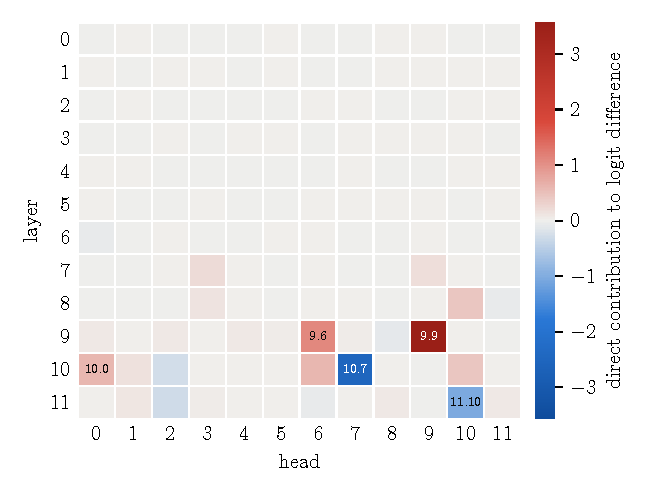
\includegraphics[width=0.5\textwidth]{figures/fig_dla_heads.pdf}
\caption{Direct logit attribution of each attention head of GPT-2 small to the logit difference of the IOI task
(summands of \eqref{eq:dla-ld}, averaged over 12 prompts). Red heads push towards the correct name and blue
heads push against it.}
\label{fig:dla}
\end{figure}

\begin{caution}
Equation \eqref{eq:dla-ld} is an exact accounting identity, and a DLA term is still not the effect of removing
the component. There are two reasons. The denominator $\scale(x_n^{(L)})$ depends on all components. And a
component also acts \emph{indirectly}, by changing what later components read. DLA sees only the direct path to
the output. A head in layer 5 that is essential for the task because head 9.9 depends on it can have a DLA of zero.
\Cref{sec:necessity} shows that this is exactly what happens in our example.
\end{caution}

\subsection{Probing}
\label{sec:probing}

The lens asks whether the \emph{answer} can be read from an intermediate activation. Probing asks the same
question for an arbitrary property \citep{alain2017understanding}. We collect a data set of pairs $(x,y)$,
where $x\in\R^d$ is an activation (say, the stream at a fixed layer and position) and $y\in\{0,1\}$ labels a
property of the input (say, whether the sentence is in the past tense). A \emph{linear probe} is a logistic
regression trained on these pairs,
\begin{equation}\label{eq:probe}
\Pr(y=1\mid x) \;=\; \frac{1}{1+\exp\!\big(-(w^\top x+b_{\mathrm{probe}})\big)},\qquad w\in\R^d,\ b_{\mathrm{probe}}\in\R .
\end{equation}
High accuracy on held-out data shows that the property is \emph{linearly decodable} from the activation.
Probes have found, among many other things, parts of speech and syntactic structure in the layers of BERT
\citep{tenney2019bert,hewitt2019structural} and the coordinates of places and the dates of events in the streams
of LLMs \citep{gurnee2024language}. \citet{belinkov2022probing} surveys the method.

A well-known case shows how much the choice of the property matters. \citet{li2023emergent} trained a
transformer to predict legal moves in the board game Othello from move sequences alone and asked whether the
state of the board can be decoded from its activations. Linear probes for the colour of each square (black,
white or empty) barely beat a baseline, and probes with one hidden layer succeeded. \citet{nanda2023emergent}
then found that a \emph{linear} probe works well once the question is rephrased relative to the player whose
turn it is: whether a square holds ``my'' piece or ``the opponent's''. The information was linear all along, in
a variable that the first study had not tried.

Three cautions govern the reading of any probing result.

\begin{enumerate}
\item \textbf{The probe may do the work itself.} A probe with enough capacity can learn the task from
any sufficiently rich input, whether or not the model has computed the property. \citet{hewitt2019designing}
propose \emph{control tasks}, in which each word type receives a random label. A good probe should reach high
accuracy on the real task and low accuracy on the control task, and the difference of the two accuracies is
called \emph{selectivity}. This is the reason for preferring linear probes: they have little capacity of their
own.
\item \textbf{Decodable does not mean used.} A probe establishes a correlation between an activation and a
label. The model may carry the information without ever reading it. To show that the model uses a direction,
we have to change the activation along it and observe the output, for example by erasing the direction
\citep{elazar2021amnesic} or by steering (\cref{sec:steering}).
\item \textbf{The probe direction need not be the model's direction.} Logistic regression chooses the $w$ that
separates the classes best, and it will exploit any other feature that happens to correlate with the label in
the data set. \citet{marks2024geometry} compare such directions with the plain difference between the two class
means and report that the latter is more often the one that changes the model's behaviour under intervention.
We return to this simple estimator in \cref{sec:lrh}.
\end{enumerate}

\begin{takeaways}
Attention patterns show from where a head reads and hide what it writes. Input attribution depends on a
baseline, and only integrated gradients are a true decomposition of the output change. The logit lens shows at
which layer an answer appears, and direct logit attribution shows which component wrote it, through the direct
path only. Probes show what is decodable, which is necessary and not sufficient for being used. In the running
example these tools point at layers 7 to 9, at the name mover heads 9.9, 9.6 and 10.0, and at the opposing heads
10.7 and 11.10.
\end{takeaways}

\begin{exercise}\label{ex:linearig}
Let $F$ be a linear function of $z$ without a constant term, so that its gradient $\nabla_{z_i}F$ is the same at
every point. Show that integrated gradients with baseline $\bar z=0$ coincide with gradient times input. Then take $n=d=1$ and $F(z)=z^2$, and show that
gradient times input is twice the integrated gradient.
\end{exercise}
\begin{exercise}\label{ex:lenslast}
Show that at $\ell=L$ the lens logits \eqref{eq:lens} are the logits of the model. Then explain why the sum of
the DLA terms of all components in layers $0,\dots,8$, together with the embeddings, is in general \emph{not}
equal to the lens logit difference at $\ell=9$.
\end{exercise}
\begin{exercise}\label{ex:probecontrol}
Suppose that a linear probe trained on the stream of layer 6 reaches 95\% accuracy for the property ``the
current token is a first name''. Describe a control experiment that shows whether this says anything
about layer 6, and predict its outcome using \eqref{eq:embed}.
\end{exercise}

\section{Features, directions and superposition}
\label{sec:features}

The methods of \cref{sec:observation} work with components that the architecture hands us: heads, layers,
positions. To say what a model \emph{represents} we need a second kind of unit, one that corresponds to a
concept. This section explains why single neurons are not that unit, and what the current working hypothesis
is.

\subsection{Features and the trouble with neurons}

We use the word \emph{feature} for a property of the input, or of the model's intermediate reasoning, that the
model represents internally because it is useful for prediction. Examples are ``the current token is a first
name'', ``this text is French'', ``the subject of the sentence is plural'' or ``this name has occurred before''.
The definition is informal on purpose. Making it precise is an open problem, and the hypotheses below are
attempts to do so.

The simplest conceivable design would give each feature its own neuron. Some neurons do behave like this. Many
do not. \citet{bricken2023monosemanticity} describe a neuron of a small language model that is active on
academic citations, on English dialogue, on HTTP requests and on Korean text. Such neurons are called
\emph{polysemantic}. Reading
them one at a time gives descriptions that are both vague and incomplete, and \citet{bolukbasi2021interpretability}
showed that the handful of strongest activations of a neuron can suggest a clean meaning that disappears when
one looks at a different data set.

For the residual stream the hope was never reasonable. By the last fact of \cref{sec:facts}, its coordinates
have no special role, so a feature has no reason to align with one of them.

\subsection{The linear representation hypothesis}
\label{sec:lrh}

If features are not coordinates, the next simplest possibility is that they are \emph{directions}.

\begin{definition}[Linear representation hypothesis, working form]\label{def:lrh}
For an activation $x\in\R^d$ at a fixed place in the model (say, the stream after a given layer) there are unit
vectors $v_1,\dots,v_N\in\R^d$, called \emph{feature directions}, and non-negative functions $f_1,\dots,f_N$ of
the input, called \emph{feature activations}, such that
\begin{equation}\label{eq:lrh}
x \;\approx\; \sum_{j=1}^{N}f_j\,v_j
\end{equation}
on all inputs of interest, where each $f_j$ measures the presence of one feature and only few of the $f_j$ are
nonzero on any single input.
\end{definition}

The hypothesis says two things: the \emph{presence} of a feature is a direction, and its \emph{strength} is the
length along that direction. It is a hypothesis about trained networks and not a theorem. The evidence for it
comes from several independent sources.

\begin{itemize}
\item \textbf{Vector arithmetic.} In word embeddings, differences between vectors encode relations. The famous
example is that the vector of \tok{king} minus that of \tok{man} plus that of \tok{woman} lies close to the
vector of \tok{queen} \citep{mikolov2013linguistic}.
\item \textbf{Linear probes.} A wide range of properties is linearly decodable (\cref{sec:probing}), including
ones as abstract as the truth of a statement \citep{marks2024geometry}. The concept activation vectors of
\citet{kim2018interpretability} apply the same idea to image classifiers.
\item \textbf{Steering.} Adding a suitable vector to the stream switches a behaviour on or off
(\cref{sec:steering}). This is causal evidence, which the first two items are not.
\item \textbf{An architectural reason.} Every component reads the stream through a linear map. A property that
is stored along a direction can be read by one row of such a map, so linear storage is the cheapest format for
whatever later layers need.
\end{itemize}

\paragraph{Estimating a direction from labelled data.} Suppose we have activations $x$ with labels
$y\in\{0,1\}$ that say whether a concept is present. The \emph{difference of means} is the vector
$\E[x\mid y=1]-\E[x\mid y=0]$, estimated by the two sample averages. Under \eqref{eq:lrh} taken as an equality
we can say exactly what it measures. By linearity of the expectation,
\begin{equation}\label{eq:diffmeans}
\E[x\mid y=1]-\E[x\mid y=0] \;=\; \sum_{j=1}^{N}\big(\E[f_j\mid y=1]-\E[f_j\mid y=0]\big)\,v_j .
\end{equation}
If the label marks the presence of feature $j$ and all other features have the same average in both classes,
only one term survives, and the difference of means is a positive multiple of $v_j$. If some other feature is
more frequent in one class, its direction is mixed in. Equation \eqref{eq:diffmeans} is therefore also a recipe
for data collection: the two classes should differ in the concept and in nothing else. Pairs of prompts that
differ in a single word, like the clean and corrupted prompts of \cref{sec:interventions}, are built for this
purpose.

\begin{caution}
The hypothesis has known exceptions. \citet{engels2025not} found that GPT-2 and Mistral 7B represent the day of
the week and the month of the year on a circle inside a two-dimensional subspace. Such a feature is not a single
direction with a strength. There are also several inequivalent ways to make the word ``linear'' precise, which
\citet{park2024linear} disentangle. \Cref{def:lrh} should be read as a productive first approximation.
\end{caution}

\subsection{Superposition: more features than dimensions}
\label{sec:superposition}

\Cref{def:lrh} does not say how large $N$ is. If the directions had to be orthogonal, we would have $N\le d$, and
a stream of width $768$ could hold $768$ features. The world contains far more than $768$ things worth
representing. The \emph{superposition hypothesis} \citep{elhage2022toy} says that networks escape this limit by
using directions that are only \emph{almost} orthogonal, and that $N$ is much larger than $d$. A related picture
for word embeddings was proposed earlier by \citet{arora2018linear}. The hypothesis rests on a geometric fact:
in high dimension there is room for a number of almost orthogonal directions that grows exponentially with $d$.

\begin{proposition}[Many almost orthogonal directions]\label{prop:jl}
Let $0<\varepsilon<1$ and let $N\ge 2$ be an integer with $N\le\exp(\varepsilon^2d/4)$. Then there are unit
vectors $v_1,\dots,v_N\in\R^d$ with $|v_i^\top v_j|\le\varepsilon$ for all $i\ne j$.
\end{proposition}
\begin{proof}
We choose the vectors at random and show that they have the property with positive probability. Let all $dN$
coordinates of $v_1,\dots,v_N$ be independent, each equal to $+1/\sqrt d$ or $-1/\sqrt d$ with probability $1/2$.
Every $v_j$ then has norm one.

\textbf{One pair.} Fix $i\ne j$. The number $d\,v_i^\top v_j$ is a sum of $d$ terms, one for each coordinate, and
each term is the product of two independent uniform random signs. Such a product is again a uniform random
sign, and the $d$ terms are independent because the coordinates are. Hoeffding's inequality
\citep[Theorem 2]{hoeffding1963probability} states that a sum of $d$ independent random variables with values in
$[-1,1]$ and mean zero is at least $\varepsilon d$ with probability at most $\exp(-(\varepsilon d)^2/(2d))$. We
use it for the sum $d\,v_i^\top v_j$ and for its negative:
\begin{align}
\Pr\big(|v_i^\top v_j|>\varepsilon\big)
&\le \Pr\big(d\,v_i^\top v_j\ge\varepsilon d\big)+\Pr\big(-d\,v_i^\top v_j\ge\varepsilon d\big) && \by{union of two events}\notag\\
&\le 2\exp\!\big(-(\varepsilon d)^2/(2d)\big) && \by{Hoeffding, twice}\notag\\
&= 2\exp\!\big(-\varepsilon^2d/2\big). && \by{since $(\varepsilon d)^2/(2d)=\varepsilon^2d/2$} \label{eq:onepair}
\end{align}

\textbf{All pairs.} There are $N(N-1)/2$ pairs $i<j$. Hence
\begin{align*}
\Pr\big(\text{some pair has }|v_i^\top v_j|>\varepsilon\big)
&\le \frac{N(N-1)}{2}\cdot 2\exp\!\big(-\varepsilon^2d/2\big) && \by{union bound and \eqref{eq:onepair}}\\
&< N^2\exp\!\big(-\varepsilon^2d/2\big) && \by{since $N(N-1)<N^2$}\\
&\le \exp\!\big(\varepsilon^2d/2\big)\exp\!\big(-\varepsilon^2d/2\big) \;=\; 1. && \by{since $N\le\exp(\varepsilon^2d/4)$}
\end{align*}
The probability that some pair violates the bound is strictly smaller than one. So there is an outcome in
which no pair violates it, and this outcome is the required family of vectors.
\end{proof}

For $d=768$ and $\varepsilon=0.3$ the proposition allows $N\le e^{17.28}$, which is more than $3\times10^7$
directions, compared with $768$ exactly orthogonal ones. The constants in the bound are far from optimal. The
point is the exponential dependence on $d$. The mechanism is easy to remember. A sum of $d$ random signs has
typical size $\sqrt d$, so two random unit vectors have an inner product of typical size $1/\sqrt d$, which is
$0.036$ for $d=768$.

Almost orthogonal is not orthogonal, and the price is \emph{interference}. If we read feature $j$ from $x$ by
projecting on $v_j$, the other active features leak into the result.

\begin{lemma}[Interference is controlled by sparsity]\label{lem:interference}
Let $v_1,\dots,v_N$ be unit vectors with $|v_i^\top v_j|\le\varepsilon$ for $i\ne j$. Let $x=\sum_{i=1}^{N}f_iv_i$,
where at most $k$ of the numbers $f_1,\dots,f_N$ are nonzero and all of them lie in $[0,1]$. Then
$|v_j^\top x-f_j|\le k\varepsilon$ for every $j$.
\end{lemma}
\begin{proof}
We expand $v_j^\top x$ and bound the terms with $i\ne j$.
\begin{align*}
|v_j^\top x-f_j| &= \Big|\sum_{i=1}^{N}f_i\,v_j^\top v_i-f_j\Big| && \by{definition of $x$}\\
&= \Big|\sum_{i\ne j}f_i\,v_j^\top v_i\Big| && \by{since $v_j^\top v_j=1$}\\
&\le \sum_{i\ne j}f_i\,|v_j^\top v_i| && \by{triangle inequality, $f_i\ge0$}\\
&\le k\varepsilon. && \by{at most $k$ nonzero terms, each at most $\varepsilon$}\qedhere
\end{align*}
\end{proof}

The lemma shows what superposition needs: \emph{sparsity}. Packing many features into few dimensions is
harmless as long as only a few of them are active at the same time, because then $k\varepsilon$ is small. Most
features of language are of this kind. Almost no text is about the Golden Gate Bridge. A nonlinearity can
then remove the remaining interference. If feature $j$ is absent, the lemma gives $v_j^\top x\le k\varepsilon$,
so $\relu(v_j^\top x-k\varepsilon)=0$: a threshold reads an absent feature as exactly absent.

\begin{figure}[t]
\centering
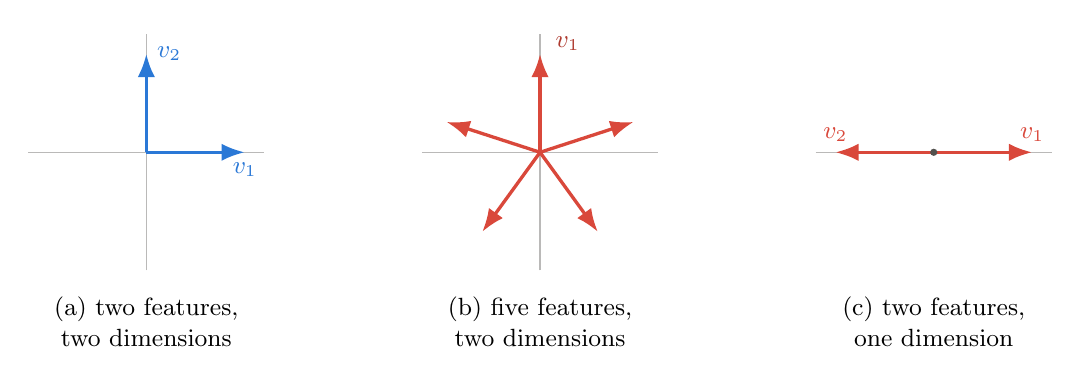
\begin{tikzpicture}[>=Latex, font=\small]
% panel a
\begin{scope}
\draw[tutgrey!40] (-1.5,0) -- (1.5,0); \draw[tutgrey!40] (0,-1.5) -- (0,1.5);
\draw[->, line width=1.2pt, tutblue] (0,0) -- (1.25,0) node[below] {$v_1$};
\draw[->, line width=1.2pt, tutblue] (0,0) -- (0,1.25) node[right] {$v_2$};
\node[align=center] at (0,-2.15) {(a) two features,\\ two dimensions};
\end{scope}
% panel b
\begin{scope}[xshift=5.0cm]
\draw[tutgrey!40] (-1.5,0) -- (1.5,0); \draw[tutgrey!40] (0,-1.5) -- (0,1.5);
\foreach \k in {1,...,5} {\draw[->, line width=1.2pt, tutred] (0,0) -- ({1.25*cos(90+72*(\k-1))},{1.25*sin(90+72*(\k-1))});}
\node[tutred!80!black] at (0.35,1.38) {$v_1$};
\node[align=center] at (0,-2.15) {(b) five features,\\ two dimensions};
\end{scope}
% panel c
\begin{scope}[xshift=10.0cm]
\draw[tutgrey!40] (-1.5,0) -- (1.5,0);
\draw[->, line width=1.2pt, tutred] (0,0) -- (1.25,0) node[above] {$v_1$};
\draw[->, line width=1.2pt, tutred] (0,0) -- (-1.25,0) node[above] {$v_2$};
\fill[tutgrey] (0,0) circle (1.3pt);
\node[align=center] at (0,-2.15) {(c) two features,\\ one dimension};
\end{scope}
\end{tikzpicture}
\caption{Feature directions without superposition (a) and with superposition (b, c). In (b) neighbouring
directions of the pentagon have inner product $\cos 72^\circ\approx0.31$, and the others have
$\cos 144^\circ\approx-0.81$. In (c) the two directions are
antipodal, with inner product $-1$. Both arrangements appear as solutions of the toy model of
\citet{elhage2022toy}.}
\label{fig:superposition}
\end{figure}

\subsection{A toy model that can be solved by hand}
\label{sec:toy}

\citet{elhage2022toy} study superposition in the smallest network that can show it. We describe their model in
the notation of \cref{def:lrh}. They write $x$ for our $f$ and $h$ for our $x$, and their sparsity parameter is our $1-\delta$.

There are $N$ features with activations $f=(f_1,\dots,f_N)$. The features are independent. Each $f_j$ is zero
with probability $1-\delta$ and uniformly distributed on $[0,1]$ with probability $\delta$, so a small $\delta$
means sparse features. The model compresses $f$ into $d<N$ dimensions and tries to recover it:
\begin{equation}\label{eq:toy}
x \;=\; Wf\in\R^d,\qquad \hat f \;=\; \relu\big(W^\top x+b_{\mathrm{toy}}\big)\in\R^N,\qquad
\text{loss} \;=\; \E\sum_{j=1}^{N}\big(f_j-\hat f_j\big)^2 ,
\end{equation}
with a weight matrix $W\in\R^{d\times N}$ and a bias $b_{\mathrm{toy}}\in\R^N$. Column $j$ of $W$ is the direction
that the model assigns to feature $j$. The original model also weights each feature by an importance, which we
set to one.

We work out the case of $N=2$ features and $d=1$ dimension completely. The model has one number $x$ to store
two features. We compare two ways of using it.

\begin{itemize}
\item \textbf{Dedicated solution.} $W=(1,\ 0)$ and $b_{\mathrm{toy}}=(0,\ \delta/2)$. The model stores feature $1$
and ignores feature $2$, for which it always outputs the constant $\delta/2$.
\item \textbf{Antipodal solution.} $W=(1,\ -1)$ and $b_{\mathrm{toy}}=(0,\ 0)$. The model stores the difference
$x=f_1-f_2$, as in \cref{fig:superposition}(c). For example, the input $f=(0.6,\ 0.2)$ is stored as $x=0.4$ and read
back as $\hat f=(0.4,\ 0)$.
\end{itemize}

\begin{proposition}[Superposition wins when features are sparse]\label{prop:toy}
In the model \eqref{eq:toy} with $N=2$, $d=1$ and $0<\delta\le1$, the dedicated solution has loss
$\delta/3-\delta^2/4$ and the antipodal solution has loss $\delta^2/3$. The antipodal solution has the smaller
loss if and only if $\delta<4/7$.
\end{proposition}
\begin{proof}
We use that a variable which is uniform on $[0,1]$ has mean $1/2$ and second moment $1/3$. Hence
$\E f_2=\delta/2$ and $\E f_2^2=\delta/3$.

\textbf{Dedicated solution.} Here $x=f_1$, so $\hat f_1=\relu(f_1)=f_1$ and $\hat f_2=\relu(\delta/2)=\delta/2$.
\begin{align*}
\text{loss} &= \E\big(f_1-f_1\big)^2+\E\big(f_2-\delta/2\big)^2 && \by{inserting $\hat f_1$ and $\hat f_2$}\\
&= \E f_2^2-\delta\,\E f_2+\delta^2/4 && \by{expanding the square}\\
&= \delta/3-\delta^2/2+\delta^2/4 \;=\; \delta/3-\delta^2/4. && \by{since $\E f_2=\delta/2$, $\E f_2^2=\delta/3$}
\end{align*}

\textbf{Antipodal solution.} Here $x=f_1-f_2$, so $\hat f_1=\relu(f_1-f_2)$ and $\hat f_2=\relu(f_2-f_1)$. If
$f_2=0$, then $\hat f_1=f_1$ and $\hat f_2=\relu(-f_1)=0=f_2$, and the error is zero. The same holds if $f_1=0$.
The only inputs with an error are those with both features active, which has probability $\delta^2$. Let both
be active and let $f_1\ge f_2$. Then $\hat f_1=f_1-f_2$ and $\hat f_2=0$, so both errors equal $f_2$ and the
squared error is $2f_2^2=2\min(f_1,f_2)^2$. For $f_2\ge f_1$ we obtain the same expression by symmetry. Given that
both features are active, $f_1$ and $f_2$ are independent and uniform on $[0,1]$, so
$\Pr(\min(f_1,f_2)>u)=(1-u)^2$ and the minimum has density $2(1-u)$ on $[0,1]$.
\begin{align*}
\text{loss} &= \delta^2\cdot 2\int_0^1u^2\cdot 2(1-u)\,du && \by{error only if both active}\\
&= \delta^2\cdot 4\Big(\frac13-\frac14\Big) \;=\; \frac{\delta^2}{3}. && \by{since $\textstyle\int_0^1u^2du=\frac13$, $\int_0^1u^3du=\frac14$}
\end{align*}

\textbf{Comparison.} For $\delta>0$,
\begin{align*}
\frac{\delta^2}{3}<\frac{\delta}{3}-\frac{\delta^2}{4}
\;&\Longleftrightarrow\; \frac{\delta}{3}+\frac{\delta}{4}<\frac13 && \by{dividing by $\delta$, rearranging}\\
&\Longleftrightarrow\; \delta<\frac47. && \by{since $\tfrac13+\tfrac14=\tfrac{7}{12}$}\qedhere
\end{align*}
\end{proof}

\begin{intuition}
The antipodal solution is wrong only when both features are present at once, and in that case it is badly
wrong. The dedicated solution is always exactly right about one feature and always ignorant about the other.
If features are rare, the collisions are rarer still ($\delta^2$ against $\delta$), and it pays to store both.
Superposition is a bet on sparsity.
\end{intuition}

Neither of the two solutions needs to be the global minimum of the loss, and the proposition only compares the
two strategies. \citet{elhage2022toy} minimise the loss numerically for larger $N$ and $d$ and find the same
transition. When the features are dense, the model stores the $d$ most important ones in orthogonal directions
and drops the rest. As the features become sparser, it stores more and more of them, in regular arrangements
such as antipodal pairs and the pentagon of \cref{fig:superposition}(b).

\subsection{Consequences for interpretability}

If superposition is how networks store features, three conclusions follow.

\begin{itemize}
\item \textbf{Polysemantic neurons are expected.} With $N$ much larger than the number of neurons, the feature
directions cannot all be aligned with the neuron basis. Each neuron then has a nonzero component along many
feature directions and responds to all of the corresponding features.
\item \textbf{The right unit of analysis has to be found.} The features are directions that no part of the
architecture labels for us. \citet{gurnee2023finding} show both situations in real models: some features sit in
single neurons, and others are spread over many.
\item \textbf{Finding them is a sparse recovery problem.} We observe many activation vectors $x$. We look for a
set of directions, more numerous than the dimension, such that each $x$ is a combination of a few of them. This
problem is known as sparse dictionary learning, and \cref{sec:sae} describes the method that is currently used
for it.
\end{itemize}

\Cref{lem:interference} concerns the \emph{storage} of features. Whether and how networks can also
\emph{compute} with features in superposition is a separate question with its own theory
\citep{hanni2024mathematical,adler2024complexity}.

\begin{takeaways}
The working hypothesis is that features are directions, and that their activations are lengths along these
directions. High-dimensional spaces contain exponentially many almost orthogonal directions, so a network can
store far more features than it has dimensions. The interference between them is small as long as few features
are active at once. Neurons are then mixtures of many features, and the features have to be recovered by sparse
dictionary learning.
\end{takeaways}

\begin{exercise}\label{ex:triangle}
Three features are stored in $d=2$ dimensions along unit vectors at mutual angles of $120^\circ$. Show that
$v_i^\top v_j=-1/2$ for $i\ne j$. Show that the read-out $\hat f_j=\relu(v_j^\top x)$ recovers $f$ exactly whenever
at most one feature is active.
\end{exercise}
\begin{exercise}\label{ex:bound}
Evaluate the bound of \cref{prop:jl} for $d=4096$ with $\varepsilon=0.1$ and with $\varepsilon=0.2$. For which
$k$ does \cref{lem:interference} then guarantee an interference below $1/2$?
\end{exercise}
\begin{exercise}\label{ex:nobias}
In \cref{prop:toy}, replace the bias of the dedicated solution by $b_{\mathrm{toy}}=(0,0)$. Compute the loss and
show that the antipodal solution is now better for every $\delta<1$. What does the bias $\delta/2$ achieve?
\end{exercise}

\section{Sparse autoencoders}
\label{sec:sae}

\Cref{sec:features} ended with a problem: given many activation vectors, find a large set of directions such
that every vector is a combination of a few of them. The \emph{sparse autoencoder} (SAE) is the tool that the
field currently uses for this. It was introduced to interpretability by \citet{bricken2023monosemanticity} and
\citet{cunningham2024sparse} and has since been scaled to production models
\citep{templeton2024scaling,gao2025scaling}.

\subsection{Definition}

We fix a place in the model, for instance the residual stream after layer 6, and collect its activation
$x\in\R^d$ at every token of a large text corpus. An SAE with $m$ \emph{latents}, where $m$ is much larger than
$d$, consists of an encoder and a decoder,
\begin{equation}\label{eq:sae}
f(x) \;=\; \relu\big(\Wenc\,(x-\bdec)+\benc\big)\in\R^m,\qquad
\hat x(x) \;=\; \Wdec\,f(x)+\bdec\in\R^d ,
\end{equation}
with $\Wenc\in\R^{m\times d}$, $\Wdec\in\R^{d\times m}$, $\benc\in\R^m$ and $\bdec\in\R^d$. We write $\Wdec[j]\in\R^d$
for column $j$ of the decoder and call it the \emph{dictionary direction} of latent $j$. The columns are kept at
unit norm. The parameters are trained to minimise
\begin{equation}\label{eq:saeloss}
\text{loss} \;=\; \E\Big[\big\|x-\hat x(x)\big\|^2+\lambda\sum_{j=1}^{m}f_j(x)\Big],\qquad\lambda>0,
\end{equation}
where the expectation is over the collected activations. The first term asks for a faithful reconstruction.
The second term is the sum of the absolute values of the entries of $f(x)$, since $f_j(x)\ge0$. It is known as
an L1 penalty, and it pushes most latents to zero.
\Cref{fig:sae} (left) shows the architecture.

Comparing $\hat x(x)=\bdec+\sum_jf_j(x)\,\Wdec[j]$ with \eqref{eq:lrh}, we see what is hoped for: the dictionary
directions $\Wdec[j]$ should be the feature directions $v_j$, and the latent activations should be the feature
activations. We keep the two notions apart by name. A \emph{latent} is a unit of an SAE, which we can compute.
A \emph{feature} is a property that the model represents, which we want to know. Whether a given latent
corresponds to a feature is an empirical question in every single case.

The method descends from sparse coding in neuroscience \citep{olshausen1997sparse}. Classical sparse coding
solves a separate optimisation problem for the coefficients of each data point. An SAE replaces this by a single
learned encoder, which makes it cheap enough for billions of activations. Dictionary sizes in published work
range from a few thousand latents to $2^{25}\approx34$ million for a production model
\citep{templeton2024scaling}.

\begin{figure}[t]
\centering
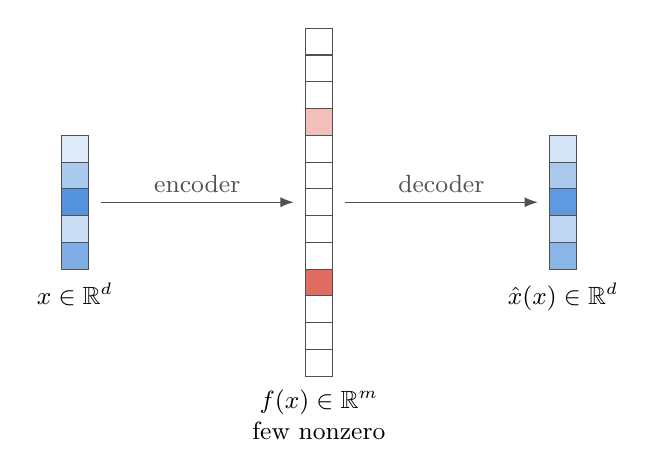
\begin{tikzpicture}[>=Latex, font=\small]
\foreach \y/\c in {0/60,1/25,2/80,3/40,4/15} {\draw[tutgrey, fill=tutblue!\c] (0,0.34*\y) rectangle +(0.34,0.34);}
\node[below, align=center] at (0.17,-0.05) {$x\in\R^d$};
\foreach \y in {0,...,12} {\draw[tutgrey, fill=white] (3.1,0.34*\y-1.36) rectangle +(0.34,0.34);}
\draw[tutgrey, fill=tutred!80] (3.1,0.34*3-1.36) rectangle +(0.34,0.34);
\draw[tutgrey, fill=tutred!35] (3.1,0.34*9-1.36) rectangle +(0.34,0.34);
\node[below, align=center] at (3.27,-1.41) {$f(x)\in\R^m$\\ few nonzero};
\foreach \y/\c in {0/55,1/30,2/75,3/40,4/20} {\draw[tutgrey, fill=tutblue!\c] (6.2,0.34*\y) rectangle +(0.34,0.34);}
\node[below, align=center] at (6.37,-0.05) {$\hat x(x)\in\R^d$};
\draw[->, tutgrey] (0.5,0.85) -- node[above] {encoder} (2.95,0.85);
\draw[->, tutgrey] (3.6,0.85) -- node[above] {decoder} (6.05,0.85);
\end{tikzpicture}
\hfill
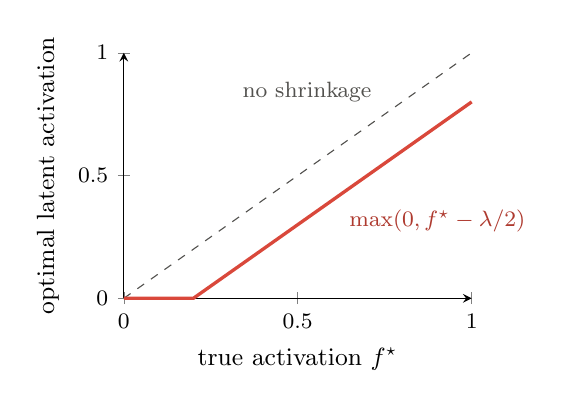
\begin{tikzpicture}
\begin{axis}[width=6.0cm, height=4.7cm, xmin=0, xmax=1, ymin=0, ymax=1, axis lines=left,
  xlabel={true activation $f^\star$}, ylabel={optimal latent activation}, label style={font=\small},
  tick label style={font=\footnotesize}, xtick={0,0.5,1}, ytick={0,0.5,1}, clip=false]
\addplot[dashed, tutgrey, domain=0:1, samples=2] {x};
\addplot[tutred, very thick, domain=0:1, samples=201] {max(0,x-0.2)};
\node[font=\footnotesize, tutgrey, anchor=south east] at (axis cs:0.74,0.76) {no shrinkage};
\node[font=\footnotesize, tutred!80!black, anchor=north west] at (axis cs:0.62,0.40) {$\max(0,f^\star-\lambda/2)$};
\end{axis}
\end{tikzpicture}
\caption{Left: a sparse autoencoder maps an activation to a much longer vector with few nonzero entries and
back. Right: the latent activation that minimises reconstruction error plus L1 penalty
(\cref{prop:shrink}, drawn for $\lambda=0.4$) lies below the true activation by $\lambda/2$.}
\label{fig:sae}
\end{figure}

\subsection{What the sparsity penalty does to the activations}

The penalty in \eqref{eq:saeloss} is a compromise. What we want to keep small is the \emph{number} of active
latents. That number is not differentiable, and the sum of the activations is used in its place. The price of
the substitute can be computed exactly in the simplest situation.

\begin{proposition}[Shrinkage]\label{prop:shrink}
Let $v\in\R^d$ be a unit vector and let $x=f^\star v$ with $f^\star\ge0$. Among all $f\ge0$, the value that
minimises $\|x-fv\|^2+\lambda f$ is
\[
f \;=\; \max\big(0,\ f^\star-\lambda/2\big).
\]
\end{proposition}
\begin{proof}
Since $\|v\|=1$, we have $\|x-fv\|^2=\|(f^\star-f)\,v\|^2=(f^\star-f)^2$. We therefore minimise
$(f^\star-f)^2+\lambda f$ over $f\ge0$. This function of $f$ is convex, and its derivative is
\begin{equation}\label{eq:shrinkderiv}
\frac{d}{df}\Big((f^\star-f)^2+\lambda f\Big) \;=\; -2\,(f^\star-f)+\lambda .
\end{equation}
If $f^\star\ge\lambda/2$, the derivative \eqref{eq:shrinkderiv} vanishes at $f=f^\star-\lambda/2\ge0$, which is
then the minimiser. If $f^\star<\lambda/2$, the derivative \eqref{eq:shrinkderiv} is at least
$\lambda-2f^\star>0$ for all $f\ge0$, so the function is increasing on $[0,\infty)$ and the minimiser is $f=0$.
\end{proof}

So a latent that fires for the right reason is still reported too small, by $\lambda/2$, and weak features are
silenced completely (\cref{fig:sae}, right). The reconstruction $\hat x$ is systematically too short. This effect
is called shrinkage or feature suppression \citep{wright2024addressing}. Current architectures avoid it by
separating the decision \emph{whether} a latent is active from the estimate of \emph{how strongly}.

\begin{itemize}
\item \textbf{TopK} \citep{gao2025scaling}. The $\relu$ in \eqref{eq:sae} is replaced by an operation that keeps
the $k$ largest entries and sets the others to zero. The number of active latents is then exactly $k$, and the
penalty is dropped.
\item \textbf{JumpReLU} \citep{rajamanoharan2024jumping}. Each latent has a learned threshold $\theta_j>0$.
An entry passes unchanged if it exceeds $\theta_j$ and is set to zero otherwise. The loss penalises the number
of active latents directly, and the missing gradient is replaced by an estimate.
\item \textbf{Gated} \citep{rajamanoharan2024improving}. One part of the encoder decides which latents are
active, and another part estimates their magnitudes.
\end{itemize}

\subsection{How to judge a dictionary}
\label{sec:saeeval}

An SAE has no ground truth to be compared with, since the true features are unknown. It is judged by several
numbers at once.

\begin{enumerate}
\item \textbf{Reconstruction.} The fraction of variance unexplained,
$\E\|x-\hat x(x)\|^2\,/\,\E\|x-\E x\|^2$, should be small.
\item \textbf{Sparsity.} The average number of nonzero latents per activation, usually called the L0 of the SAE, should be
small compared with $d$. Published dictionaries have values from about ten to a few hundred.
\item \textbf{Effect on the model.} One runs the model with $x$ replaced by $\hat x(x)$ and measures how much the
next-token loss increases. This matters because the model does not care equally about all directions of $x$. A
small reconstruction error can sit in exactly the direction that a later layer reads.
\item \textbf{Health.} \emph{Dead} latents never fire, and \emph{dense} latents fire on a large share of all
tokens. Both are wasted capacity.
\item \textbf{Interpretability.} For a sample of latents, a human or a language model writes a short
description of the texts on which the latent fires. The description is scored by how well it predicts the
activations on new texts \citep{bills2023language}.
\end{enumerate}

Items 1 and 2 trade off against each other, so two SAEs can only be compared along a whole curve.
\citet{karvonen2025saebench} collect these and further tests in a benchmark.

\subsection{Reading a single latent}
\label{sec:latent}

Suppose a latent has passed these tests. Three views are combined to understand it.

\begin{itemize}
\item \textbf{Where it fires.} One reads text on which the latent is active. The examples should be sampled over
the whole range of activations. The strongest ones alone give too clean a picture.
\item \textbf{What it writes.} By \cref{prop:dla}, adding a multiple of $\Wdec[j]$ to the final stream changes
the logit of token $t$ in proportion to $W_U[t]^\top(\Wdec[j]-\mean(\Wdec[j])\,\one)$. Sorting the vocabulary by
this number shows which tokens the latent promotes directly.
\item \textbf{What happens when it is changed.} One runs the model while holding $f_j$ at zero or at a large
value and adds the corresponding change of $\hat x$ to the stream. This is an intervention, and it is the only
one of the three views that tests whether the model uses the direction.
\end{itemize}

The best-known example is from \citet{templeton2024scaling}, who trained SAEs with up to $2^{25}$ latents on a
middle layer of the production model Claude 3 Sonnet. One latent fired on mentions and pictures of the Golden
Gate Bridge. When the authors clamped it to ten times its maximal observed value, the model began to describe
itself as the Golden Gate Bridge. Open dictionaries exist for open models, for example Gemma Scope for all layers
of Gemma 2 \citep{lieberum2024gemma}, and can be browsed on Neuronpedia \citep{lin2023neuronpedia}.

\subsection{What a sparse autoencoder does not give}

The appeal of SAEs is that they produce units with readable descriptions without any labels. The following
limits are established by now and have to be kept in mind when using them.

\begin{caution}
\textbf{The reconstruction is imperfect.} An analysis in terms of latents describes $\hat x$, and the remainder
$x-\hat x$ often matters for the output (item 3 of \cref{sec:saeeval}).

\textbf{The dictionary is not canonical.} The latents depend on the dictionary size. A latent of a small SAE
tends to split into several more specific latents in a larger one \citep{bricken2023monosemanticity}, and no
size is the correct one \citep{leask2025sparse}. They also depend on the random seed
\citep{paulo2025sparse}. A general latent can fail to fire on cases that a more specific latent has taken over,
which is called absorption \citep{chanin2024absorption}.

\textbf{Readable latents do not prove learned structure.} \citet{heap2025sparse} trained SAEs on transformers
with random weights and obtained latents with similar automatic interpretability scores. Part of the
sparse structure comes from the input text and not from anything the network has learned.

\textbf{Usefulness has to be shown per task.} On supervised tasks with labels, simple baselines are hard to
beat. \citet{kantamneni2025sparse} found no consistent advantage of probes on SAE latents over probes on raw
activations, and \citet{wu2025axbench} found that steering with SAE latents was weaker than simple alternatives.
\end{caution}

None of this makes SAEs useless. They remain the main tool for discovering concepts that one did not think of in
advance. It does mean that a latent is a hypothesis about the model, to be tested with the interventions of
\cref{sec:interventions}.

\subsection{Relatives: transcoders and crosscoders}
\label{sec:transcoders}

An SAE reconstructs an activation from itself. Two variants change what is reconstructed from what.
A \emph{transcoder} \citep{dunefsky2024transcoders} has the same form as \eqref{eq:sae}, and it is trained to
predict the \emph{output} of an MLP layer from the \emph{input} of that layer. It is a sparse, wide replacement
of the MLP. Its use is in circuit analysis. Between an SAE latent in one layer and an SAE latent in a later
layer lies a nonlinear MLP, and their interaction is hard to describe. With transcoders, the path from one
latent to the next passes only through linear maps once the attention patterns and the scales in $\LN$ are
held fixed, and it can be read from the weights. \Cref{sec:featurecircuits} builds on this. A \emph{crosscoder} \citep{lindsey2024crosscoders}
uses one set of latents to reconstruct several activations at once, either several layers of one model or the
same layer of two models. The second use allows one to ask what changed between a model and its fine-tuned
version.

\begin{takeaways}
A sparse autoencoder rewrites an activation as a sparse, non-negative combination of many learned directions.
The L1 penalty biases activations downward, which TopK and JumpReLU variants avoid. A dictionary is judged
by reconstruction, sparsity, effect on the model and interpretability together. Its latents are candidate
features. They depend on training choices, they leave an unexplained remainder, and they need causal tests.
\end{takeaways}

\begin{exercise}\label{ex:normconstraint}
Consider the loss \eqref{eq:saeloss} without the constraint that the columns of $\Wdec$ have unit norm. Show
that multiplying column $j$ of $\Wdec$ by $2$ and dividing row $j$ of $\Wenc$ and entry $j$ of $\benc$ by $2$
leaves the reconstruction unchanged and reduces the penalty. What would training do without the constraint?
\end{exercise}
\begin{exercise}\label{ex:fvu}
In the setting of \cref{prop:shrink}, let $f^\star$ be uniform on $[0,1]$ and $\lambda=0.4$. Compute the mean
squared reconstruction error $\E\,(f^\star-f)^2$ of the optimal $f$.
\end{exercise}
\begin{exercise}\label{ex:ggb}
The ten strongest activations of a latent are all on text about the Golden Gate Bridge. Name two further
observations and one intervention that you would require before calling it a ``Golden Gate Bridge feature''.
\end{exercise}

\section{Causal interventions}
\label{sec:interventions}

Everything so far has been observation. We recorded activations and found structure in them. Structure in
activations shows what \emph{could} be used by the model. To learn what \emph{is} used, we have to change an
activation and see whether the output changes. A neural network is an unusually good object for this kind of
experiment. We can set any internal quantity to any value, rerun the rest of the computation exactly, and
repeat as often as we like.

\subsection{Interventions and ablations}

\begin{definition}[Intervention]\label{def:intervention}
A \emph{node} $g$ is any intermediate quantity of the model: the residual stream at one layer and position, the
output of one head, one neuron, one SAE latent. The components of \cref{prop:dla} are examples. We write $g(\clean)$ for the value of the node when the model
runs on a prompt called $\clean$, and $M(\clean)$ for a scalar measure of the output on that prompt, the
\emph{metric}. For a value of the same shape as $g$, the \emph{intervened run} computes everything before the
node as usual, overwrites the node with the given value, and recomputes everything after it. We write
\[
M\big(\clean \mid g\leftarrow\text{value}\big)
\]
for the metric of the intervened run.
\end{definition}

Throughout this section the metric is the logit difference \eqref{eq:ld}. The simplest interventions remove a
node and are called \emph{ablations}. They differ in the value that takes the place of the node.

\begin{center}\small
\begin{tabular}{@{}lp{0.42\textwidth}p{0.38\textwidth}@{}}
\toprule
Ablation & Value written to the node & Main weakness \\
\midrule
zero & $0$ & zero can be far from every value the node normally takes \\
mean & average of the node over a reference set of prompts & the average may be a value that never occurs \\
resample & value of the node on another, randomly chosen prompt & noisy, has to be averaged over many draws \\
\bottomrule
\end{tabular}
\end{center}

\begin{caution}
An ablation compares the model with a counterfactual model, and the replacement value defines the
counterfactual. Zero ablation of a head that always writes roughly the same large vector destroys that constant
contribution, on which later layers may rely for reasons unrelated to the task. The measured drop then says
little about the task. Mean and resample ablation keep such constant parts intact and remove only what varies
between prompts. Every ablation result should be reported together with the replacement value that was used.
\end{caution}

\subsection{Activation patching}
\label{sec:patching}

\begin{figure}[t]
\centering
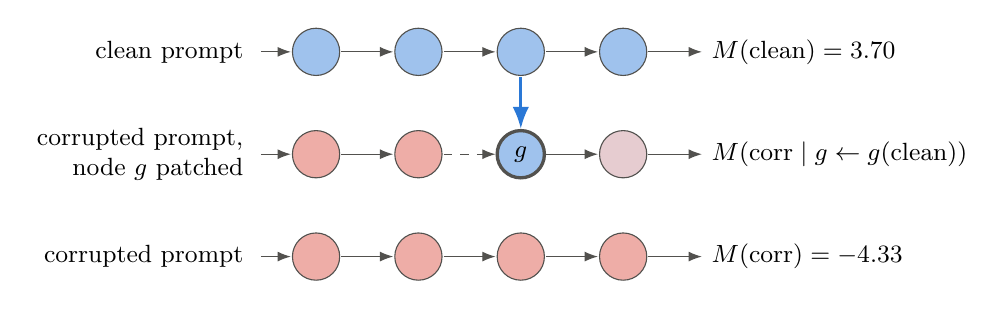
\begin{tikzpicture}[>=Latex, font=\small, n/.style={circle, draw=tutgrey, minimum size=6mm, inner sep=0pt, fill=#1}]
\def\rowa{0} \def\rowb{-1.3} \def\rowc{-2.6}
% clean row
\node[anchor=east] at (2.2,\rowa) {clean prompt};
\foreach \x in {3,4.3,5.6,6.9} {\node[n=tutblue!45] at (\x,\rowa) {};}
\draw[->,tutgrey] (2.3,\rowa) -- (2.68,\rowa);
\foreach \x in {3.32,4.62,5.92} {\draw[->,tutgrey] (\x,\rowa) -- +(0.66,0);}
\draw[->,tutgrey] (7.22,\rowa) -- (7.9,\rowa) node[right, text=black] {$M(\clean)=3.70$};
% patched row
\node[anchor=east, align=right] at (2.2,\rowb) {corrupted prompt,\\ node $g$ patched};
\node[n=tutred!45] at (3,\rowb) {}; \node[n=tutred!45] at (4.3,\rowb) {};
\node[n=tutblue!45, line width=1.2pt] (pg) at (5.6,\rowb) {$g$};
\node[n=tutblue!25!tutred!30] at (6.9,\rowb) {};
\draw[->,tutgrey] (2.3,\rowb) -- (2.68,\rowb);
\draw[->,tutgrey] (3.32,\rowb) -- +(0.66,0);
\draw[->,tutgrey, dashed] (4.62,\rowb) -- +(0.66,0);
\draw[->,tutgrey] (5.92,\rowb) -- +(0.66,0);
\draw[->,tutgrey] (7.22,\rowb) -- (7.9,\rowb) node[right, text=black] {$M(\corr\mid g\leftarrow g(\clean))$};
\draw[->, line width=1.1pt, tutblue] (5.6,-0.32) -- (pg.north);
% corrupted row
\node[anchor=east] at (2.2,\rowc) {corrupted prompt};
\foreach \x in {3,4.3,5.6,6.9} {\node[n=tutred!45] at (\x,\rowc) {};}
\draw[->,tutgrey] (2.3,\rowc) -- (2.68,\rowc);
\foreach \x in {3.32,4.62,5.92} {\draw[->,tutgrey] (\x,\rowc) -- +(0.66,0);}
\draw[->,tutgrey] (7.22,\rowc) -- (7.9,\rowc) node[right, text=black] {$M(\corr)=-4.33$};
\end{tikzpicture}
\caption{Activation patching in the denoising direction. The model runs on the corrupted prompt. One node $g$ is
overwritten with its value from the clean run, and everything after it is recomputed. If the metric moves from
$M(\corr)$ towards $M(\clean)$, the node carries information that distinguishes the two prompts.}
\label{fig:patching-schema}
\end{figure}

Activation patching refines resample ablation by choosing the other prompt deliberately
\citep{vig2020investigating,wang2023interpretability}. The causal tracing of \citet{meng2022locating} is a
variant in which the corrupted run is produced by adding noise to the embeddings of some tokens. We prepare two prompts of equal length that differ in exactly
the aspect we want to study. In the running example,
\begin{center}
\begin{tabular}{@{}ll@{}}
$\clean$: & \tok{When Mary and John went to the store, John gave a drink to} \\
$\corr$: & \tok{When Mary and John went to the store, Mary gave a drink to}
\end{tabular}
\end{center}
The corrupted prompt differs in one token, the second occurrence of the subject, and its correct continuation is
the other name. Averaged over our 12 pairs of prompts, $M(\clean)=3.70$ and $M(\corr)=-4.33$, where the metric is
always the logit difference in favour of the name that is correct for the clean prompt. The two values are not
mirror images of each other, because in the corrupted prompts the repeated name is the one that was mentioned
first. All effects below are computed from metrics that are averaged over the 12 pairs. The two runs are $8.04$
logits apart (computed from the unrounded values).

We now run the model on one prompt and overwrite a single node with its value from the other run
(\cref{fig:patching-schema}). There are two directions.

\begin{definition}[Denoising and noising]\label{def:patching}
The \emph{denoising} effect of a node $g$ is the fraction of the gap that is restored when the corrupted run
receives the clean value of $g$,
\begin{equation}\label{eq:denoise}
\frac{M\big(\corr \mid g\leftarrow g(\clean)\big)-M(\corr)}{M(\clean)-M(\corr)} .
\end{equation}
The \emph{noising} effect of $g$ is the fraction of the gap that is lost when the clean run receives the
corrupted value of $g$,
\begin{equation}\label{eq:noise}
\frac{M(\clean)-M\big(\clean \mid g\leftarrow g(\corr)\big)}{M(\clean)-M(\corr)} .
\end{equation}
\end{definition}
Both numbers are $0$ for a node that plays no role and $1$ for a node that carries the whole difference between
the two prompts.


\paragraph{Where is the information?} For a first map we take as nodes the residual stream $x_i^{(\ell)}$ at
every layer $\ell$ and position $i$. \Cref{fig:residpatch} shows the denoising effect \eqref{eq:denoise} of each
of these $12\times15$ nodes. The picture is simple, and each part of it can be explained.
\begin{itemize}
\item All positions before S2 show exactly zero. The two prompts agree up to there, and a position never sees
later tokens, so the two runs have identical streams at these positions and the patch changes nothing.
\item At S2 the effect is $1.00$ in layers $0$ to $3$. Restoring the stream at the one position where the prompts
differ, early enough, restores the clean run completely. The effect at S2 is still $0.92$ at the input of layer
$7$, falls to $0.73$ at layer $8$ and to $0.07$ at layer $9$.
\item At the last position the effect is zero through layer $6$. It is $0.40$ at the input of layer $8$ and
$0.96$ at the input of layer $9$.
\end{itemize}
So the information about which name is repeated sits at S2 until about layer $7$ and is then moved to the last
position by layers $7$ and $8$. By the third fact of \cref{sec:facts}, only attention heads can do this. The
figure therefore tells us to look for heads in layers 7 and 8 that attend from the last position to S2. The
logit lens of \cref{fig:lens} showed the answer appearing one layer later, in layer 9. The two pictures together
suggest an order of events: first the information about the repeated name arrives at the last position, then
the name movers act on it.

\begin{figure}[t]
\centering
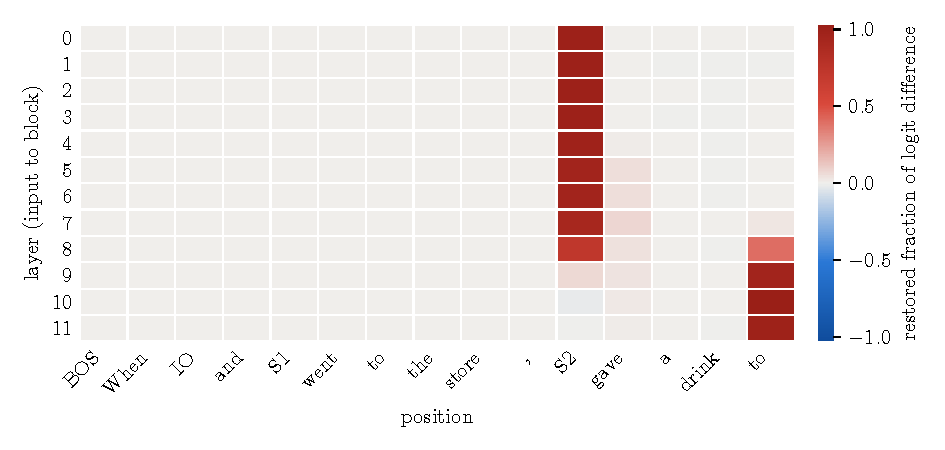
\includegraphics[width=0.86\textwidth]{figures/fig_resid_patching.pdf}
\caption{Activation patching of the residual stream of GPT-2 small on the IOI task. Each cell shows the
denoising effect \eqref{eq:denoise} of the stream at the input of one layer at one position, averaged over 12
pairs of prompts. IO is the indirect object, S1 and S2 are the two occurrences of the subject.}
\label{fig:residpatch}
\end{figure}

\begin{caution}
The corrupted prompt decides what a patching experiment can find. Ours changes which name is repeated and keeps
everything else. Components that are needed for the task and behave the same on both prompts, for example
whatever establishes that the next token should be a name at all, stay invisible. A different question requires
a different pair of prompts. \citet{zhang2024towards} and \citet{heimersheim2024use} discuss these choices in
detail.
\end{caution}

\subsection{Sufficient, necessary, direct, total}
\label{sec:necessity}

We now take the output of each attention head, at all positions, as a node. \Cref{tab:heads} lists four numbers
for twelve heads from the classes of \citet{wang2023interpretability}. The classes are explained in
\cref{sec:ioi}, and for the moment they are only labels. The first is the direct logit attribution from \cref{sec:lens}. The second
is the denoising effect \eqref{eq:denoise}. The last two describe the noising experiment in logits. The
\emph{total effect} is the numerator of \eqref{eq:noise}, which is the drop of the metric when the head receives
its corrupted output. The \emph{direct effect} is the part of this drop that comes from the head's own summand
in \eqref{eq:dla-ld}, computed with the final scale held fixed. A negative entry in the table belongs to a head
that works against the correct name: restoring it lowers the metric, and corrupting it raises the metric. The
effects of different heads do not add up to one, because the heads depend on each other. For head 9.9 the direct
effect of $7.00$ is about twice its DLA, because in the corrupted run this head writes with similar strength in
favour of the other name.

\begin{table}[t]
\centering\small
\begin{tabular}{@{}llrrrr@{}}
\toprule
 & & & denoising & \multicolumn{2}{c}{noising (logits)} \\
\cmidrule(l){5-6}
Head & Class in \citet{wang2023interpretability} & DLA & effect & direct effect & total effect \\
\midrule
9.9 & name mover & $3.57$ & $0.29$ & $7.00$ & $1.40$ \\
9.6 & name mover & $1.10$ & $0.01$ & $2.27$ & $-0.77$ \\
10.0 & name mover & $0.59$ & $0.09$ & $1.31$ & $0.57$ \\
10.7 & negative name mover & $-2.52$ & $-0.52$ & $-4.62$ & $-3.83$ \\
11.10 & negative name mover & $-1.05$ & $-0.28$ & $-2.24$ & $-2.15$ \\
\addlinespace
8.6 & S-inhibition & $0.00$ & $0.37$ & $0.01$ & $1.55$ \\
8.10 & S-inhibition & $0.44$ & $0.34$ & $0.73$ & $1.51$ \\
7.9 & S-inhibition & $0.19$ & $0.22$ & $0.42$ & $1.17$ \\
7.3 & S-inhibition & $0.22$ & $0.14$ & $0.42$ & $0.96$ \\
\addlinespace
5.5 & induction & $0.00$ & $0.33$ & $0.00$ & $1.46$ \\
6.9 & induction & $0.00$ & $0.15$ & $0.00$ & $0.37$ \\
3.0 & duplicate token & $0.00$ & $0.15$ & $0.00$ & $0.45$ \\
\bottomrule
\end{tabular}
\caption{Four views of twelve attention heads of GPT-2 small on the IOI task, averaged over 12 pairs of prompts.
DLA is in logits, the denoising effect is a fraction of the gap of $8.04$ logits between the clean and the
corrupted run, and the two noising columns are in logits. The classes are those assigned by
\citet{wang2023interpretability}.}
\label{tab:heads}
\end{table}

The table contains three lessons that hold far beyond this example.

\paragraph{Lesson 1: direct attribution misses the early part of a mechanism.} Heads 8.6, 5.5, 6.9 and 3.0 have a
DLA of zero. They write nothing in the direction that separates the two names at the output. Yet corrupting head 8.6 or head 5.5 alone costs
about $1.5$ logits. These heads matter through what later heads do with their output. Only an intervention
reveals them.

\paragraph{Lesson 2: the total effect can be much smaller than the direct effect.} Corrupting the name mover 9.9
removes $7.00$ logits of direct contribution, and the metric drops by only $1.40$. Four fifths of the damage is
undone by the layers after it. For head 9.6 the total effect is even negative: the model does slightly better
when this helpful head is corrupted. \citet{wang2023interpretability} observed the same phenomenon and found
heads that take over when the name movers are removed, which they call backup name movers.
\citet{mcgrath2023hydra} studied such compensation systematically under the name \emph{hydra effect}. The
consequence is uncomfortable: removing a component and seeing little change does not show that the component
is unimportant.

\paragraph{Lesson 3: noising and denoising answer different questions.} Denoising asks whether the clean value
of one node is \emph{sufficient} to move a corrupted run towards the clean behaviour. Noising asks whether the
clean value of one node is \emph{necessary} for the clean behaviour. If several components do the same job in
parallel, each is sufficient and none is necessary. If several components are needed jointly, each is necessary
and none is sufficient. \Cref{ex:andor} makes this exact in a model with two nodes.

\paragraph{Paths.} Patching a node changes everything downstream of it. To learn through \emph{which} later
components a node acts, we patch along selected paths only. For example, to measure the effect of head 8.6
that passes through head 9.9, we recompute the input of head 9.9 with the corrupted output of head 8.6 and
keep the clean value on every other path. This is \emph{path patching}
\citep{wang2023interpretability,goldowskydill2023localizing}. The direct effect in \cref{tab:heads} is the
special case of the path that leads straight to the output.

\begin{remark}[A clash of terminology]
In causal mediation analysis \citep{pearl2001direct,vig2020investigating} the treatment is the change of the
\emph{input}, and the ``indirect effect'' through a mediating node is the part of the change of the output that
passes through that node. This is what activation patching measures. It should not be confused with our use of
``direct'', which refers to the path from a \emph{component} to the output that avoids all later components.
\end{remark}

\subsection{Attribution patching: a linear shortcut}
\label{sec:attrpatching}

Patching costs one run of the model per node. For 144 heads this is nothing. For every neuron at every position,
or for millions of SAE latents, it is prohibitive. \emph{Attribution patching}
\citep{nanda2023attribution,syed2024attribution} estimates all patching effects at once.

Fix a node $g$ and regard the metric of the corrupted run as a function of the value written to $g$. A
first-order Taylor expansion of this function around the value $g(\corr)$ gives
\begin{equation}\label{eq:attrpatch}
M\big(\corr \mid g\leftarrow g(\clean)\big)-M(\corr) \;\approx\;
\big(g(\clean)-g(\corr)\big)^\top\,\nabla_gM(\corr),
\end{equation}
where $\nabla_gM(\corr)$ is the gradient of the metric with respect to the node, evaluated in the unmodified
corrupted run. The right-hand side needs the values of all nodes on both prompts, which two forward passes
provide, and the gradients with respect to all nodes, which a single backward pass provides. The cost no longer
depends on the number of nodes.

\Cref{fig:attrpatch} compares the estimate with the exact denoising effect for all 144 heads of the running
example. The correlation is $0.98$. The estimate identifies the same heads. Its largest errors occur for two
heads with large effects. For head 9.9 it gives $0.43$ where the exact value is $0.29$, and for head 5.5 it gives
$0.25$ where the exact value is $0.33$.

\begin{figure}[t]
\centering
\begin{minipage}[c]{0.44\textwidth}
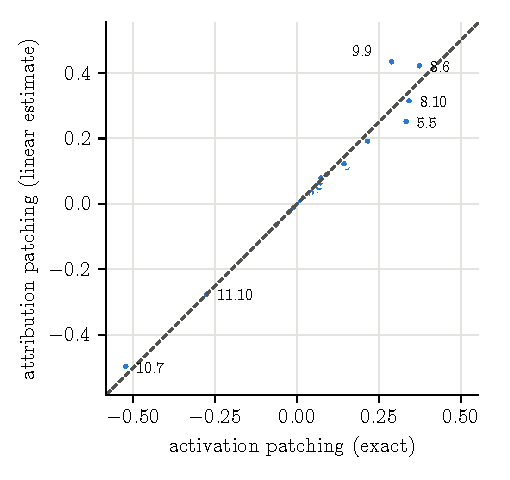
\includegraphics[width=\textwidth]{figures/fig_attr_vs_act.pdf}
\end{minipage}\hfill
\begin{minipage}[c]{0.5\textwidth}
\caption{Attribution patching against activation patching for the 144 attention heads of GPT-2 small on the IOI
task. Each dot is one head. The horizontal axis is the exact denoising effect \eqref{eq:denoise}, and the
vertical axis is the linear estimate \eqref{eq:attrpatch} divided by the same gap. Dots on the dashed diagonal
are estimated without error.}
\label{fig:attrpatch}
\end{minipage}
\end{figure}

\begin{caution}
The estimate \eqref{eq:attrpatch} is a linearisation, and it fails where the model is far from linear between
the two values. The standard example is a saturated attention pattern. If a head puts almost all its weight on
one source, the gradient with respect to the scores is almost zero, although a large change of the scores
would redirect the head completely. \citet{kramar2024atp} analyse such cases and propose corrections. In
practice the estimate serves as a fast filter, and the nodes that it selects are then patched exactly.
\end{caution}

\subsection{Steering}
\label{sec:steering}

Patching replaces an activation by one that occurred on another prompt. \emph{Steering} moves an activation
along a chosen direction and tests in this way whether the direction controls a behaviour. Let $v\in\R^d$ be a
unit vector. There are two basic operations on a stream vector $x$.
\begin{align}
\text{activation addition:}\qquad & x \;\longmapsto\; x+\eta\,v,\qquad \eta\in\R, \label{eq:actadd}\\
\text{directional ablation:}\qquad & x \;\longmapsto\; x-(v^\top x)\,v . \label{eq:dirabl}
\end{align}
The first adds the direction with a strength $\eta$ \citep{turner2023steering,rimsky2024steering,zou2023representation}.
The second removes the component of $x$ along $v$: the result has inner product
$v^\top x-(v^\top x)\,v^\top v=0$ with $v$. The direction can come from any of the earlier sections: a difference of
means \eqref{eq:diffmeans}, a probe, or a dictionary direction of an SAE.

A clear case is the study of refusal by \citet{arditi2024refusal}. Chat models are trained to refuse harmful
requests. The authors collected stream activations on harmful and on harmless instructions and took the
difference of the two means at one layer as the direction $v$. In 13 open chat models with up to 72 billion
parameters, they obtained the same two results. With \eqref{eq:dirabl} applied at all layers and positions, the
model no longer refused harmful requests. With \eqref{eq:actadd} applied at the layer where $v$ was extracted,
the model refused harmless ones. In these models the decision to refuse passes through one direction.

Results of this kind are the strongest evidence for the linear representation hypothesis of \cref{sec:lrh},
because they are causal: a direction found by observation changes the behaviour in the predicted way when it is
manipulated. They are also the basis of practical applications, since a direction that controls a behaviour
can be used to monitor or to adjust it.

\begin{caution}
Steering has its own failure modes. A large $\eta$ produces activations that the model never sees in normal
operation, and its text degrades. A direction estimated from data contains whatever else differs between the
two classes of prompts, as \eqref{eq:diffmeans} shows, so the behaviour may change for another reason than the
intended one. An evaluation should therefore measure three things: whether the intended behaviour changes,
whether unrelated behaviour stays intact, and how the method compares with simple baselines such as changing
the prompt \citep{wu2025axbench}.
\end{caution}

\subsection{Testing a hypothesis about an algorithm}
\label{sec:abstraction}

Patching single nodes localises a behaviour. A full explanation claims more: that the model implements a
particular algorithm, with named intermediate variables that are stored at particular places. \emph{Causal
abstraction} \citep{geiger2021causal,geiger2025causal} turns such a claim into an experiment. Suppose the
hypothesis says that a certain set of activations stores the variable ``the name that is repeated''. We take two
prompts with different repeated names and patch exactly these activations from the second run into the first.
The hypothesis predicts the new output: it must be what the algorithm returns when this one variable is swapped
and all others are kept. The fraction of prompt pairs on which the model agrees with the prediction is called
the interchange intervention accuracy. Causal scrubbing \citep{chan2022causal} is a related test based on
resampling.

The variable need not be stored in individual neurons or heads. Distributed alignment search
\citep{geiger2024finding} looks for it in a subspace of the stream, and finds the subspace by gradient descent on
the interchange accuracy. This added power has a price. \citet{makelov2024subspace} show that a subspace found
by optimisation can produce the predicted behaviour by activating a pathway that the model does not normally
use. The intervention then succeeds, and the explanation is still wrong. The more freedom a method has in
choosing where and how to intervene, the more carefully its result has to be checked against how the model
behaves without the intervention.

\begin{takeaways}
An intervention overwrites a node and recomputes the rest. The replacement value defines the question.
Activation patching uses the value from a minimally different prompt and localises the information that
distinguishes the two prompts. Direct effects, total effects, sufficiency and necessity are four different
quantities, and compensation by later layers can hide important components. Attribution patching approximates
all patching effects with two forward passes and one backward pass. Steering tests whether a direction controls
a behaviour.
\end{takeaways}

\begin{exercise}\label{ex:andor}
A model has two binary nodes $g_1,g_2$. On the clean prompt both are $1$, on the corrupted prompt both are $0$.
Compute the denoising effect \eqref{eq:denoise} and the noising effect \eqref{eq:noise} of $g_1$ when the metric
is (a) $M=\max(g_1,g_2)$ and (b) $M=\min(g_1,g_2)$. Relate the result to Lesson 3.
\end{exercise}
\begin{exercise}\label{ex:affine}
Show that \eqref{eq:attrpatch} holds with equality if the metric of the intervened run is an affine function of
the value written to $g$. Give an example of a node and a metric in a transformer for which this is the case.
\end{exercise}
\begin{exercise}\label{ex:projection}
Show that directional ablation \eqref{eq:dirabl} with a unit vector $v$ is linear in $x$, that applying it twice
is the same as applying it once, and that it does not change the read-out $w^\top x$ of a probe direction $w$
that is orthogonal to $v$.
\end{exercise}

\section{Circuits: from components to algorithms}
\label{sec:circuits}

The tools of the last sections answer the first two questions of \cref{sec:intro}: what is represented, and
which components matter. A \emph{circuit} is an answer to the third: how the components work together.

\subsection{What counts as a circuit}

By \cref{prop:sum}, the input of every component is a sum of the outputs of earlier components. We can
therefore draw the model as a graph. The nodes are the embeddings, the attention heads and the MLPs. There is
an edge from every component to every later component and to the output, which stands for the term that the
earlier one contributes to the input of the later one. This graph has the same structure for every model of
the same architecture. What differs is which edges carry something that matters.

\begin{definition}[Circuit]\label{def:circuit}
A \emph{circuit} for a task is a subgraph of this graph together with a description of what each of its nodes
computes on the task.
\end{definition}

A drawing of nodes and arrows is easy to produce, so the definition is only useful together with tests.
\citet{wang2023interpretability} proposed three. In all of them, components outside the set under study are
replaced by their mean over a reference distribution of prompts (mean ablation, \cref{sec:interventions}).
\begin{itemize}
\item \textbf{Faithfulness.} The circuit alone, with everything else ablated, performs about as well as the
full model.
\item \textbf{Completeness.} The circuit contains all components that take part in the behaviour. The test
removes the same subset of nodes from the circuit and from the full model and asks that the two still perform
alike, for every subset. It detects components outside the circuit that could step in.
\item \textbf{Minimality.} Every node of the circuit is needed: for each node there is a situation in which
removing it changes the performance noticeably.
\end{itemize}

\subsection{Reading an algorithm from the weights}
\label{sec:pathexp}

In sufficiently small models a circuit can be read from the weights, without running the model at all. The
cleanest case is a transformer with one layer and no MLP, studied by \citet{elhage2021mathematical}. To keep the
formulas short we also drop $\LN$ and the positional embedding. The model is then
\begin{equation}\label{eq:onelayer}
x_i^{(0)}=W_E[t_i],\qquad
x_i^{(1)}=x_i^{(0)}+\sum_{h=0}^{H-1}\sum_{j\le i}A^{0,h}_{ij}\,W_{OV}^{0,h}\,x_j^{(0)},\qquad
\logit_i(t)=W_U[t]^\top x_i^{(1)},
\end{equation}
where $W_{OV}^{0,h}$ is the matrix $W_{OV}$ of head $h$ in the single layer $0$.

\begin{proposition}[Path expansion of a one-layer attention-only transformer]\label{prop:path}
In the model \eqref{eq:onelayer},
\begin{equation}\label{eq:path}
\logit_i(t) \;=\; \underbrace{W_U[t]^\top W_E[t_i]}_{\text{direct path}}
\;+\;\sum_{h=0}^{H-1}\sum_{j\le i}A^{0,h}_{ij}\;\underbrace{W_U[t]^\top W_{OV}^{0,h}\,W_E[t_j]}_{\text{path through head }h} .
\end{equation}
\end{proposition}
\begin{proof}
We insert the stream $x_i^{(1)}$ of \eqref{eq:onelayer} into the read-out.
\begin{align*}
\logit_i(t) &= W_U[t]^\top x_i^{(0)}+\sum_{h=0}^{H-1}\sum_{j\le i}A^{0,h}_{ij}\,W_U[t]^\top W_{OV}^{0,h}\,x_j^{(0)}
&& \by{by \eqref{eq:onelayer}, linearity}\\
&= W_U[t]^\top W_E[t_i]+\sum_{h=0}^{H-1}\sum_{j\le i}A^{0,h}_{ij}\,W_U[t]^\top W_{OV}^{0,h}\,W_E[t_j].
&& \by{since $x_j^{(0)}=W_E[t_j]$}\qedhere
\end{align*}
\end{proof}

Every term of \eqref{eq:path} is an entry of a table with one row and one column per token, and each table has
a plain meaning.
\begin{itemize}
\item $W_U[t]^\top W_E[t_i]$ says how much the current token $t_i$ promotes the next token $t$ by itself. This
table approximates the statistics of pairs of adjacent tokens.
\item $W_U[t]^\top W_{OV}^{0,h}W_E[t_j]$ says how much token $t$ is promoted \emph{if} head $h$ attends to an
earlier token $t_j$.
\item Whether it attends there is decided by a third table. Without $\LN$, the score in \eqref{eq:pattern} is
proportional to $W_E[t_i]^\top W_{QK}^{0,h}W_E[t_j]$.
\end{itemize}
A one-layer attention-only transformer is therefore a sum of look-up tables of the form ``when the current
token is $t_i$ and an earlier token is $t_j$, raise or lower the probability of $t$''. The three tables can be
computed from the weights and inspected. The explanation then covers all inputs, and not only the ones that
were tried.

With two layers, the input of a head in the second layer contains the outputs of the heads in the first, and
\eqref{eq:path} acquires terms in which the tables of two heads are multiplied. This is called
\emph{composition}. It comes in three kinds, according to whether the earlier head influences the later head's
query (where it looks from), its key (what it looks for) or its value (what it moves). Composition is where
real algorithms begin.

\subsection{Induction heads}
\label{sec:induction}

The first algorithm found in this way is also the most important one known. Text is full of repetitions. If the
sequence \tok{[A][B]} has occurred and the token \tok{[A]} occurs again, then \tok{[B]} is a good guess for the
next token. Two-layer attention-only transformers implement this rule with two heads
\citep{elhage2021mathematical}, as shown in \cref{fig:induction}.

\begin{enumerate}
\item A \emph{previous-token head} in the first layer attends from every position to the position before it.
At the position of \tok{[B]} it writes into the stream the information ``the token before me was \tok{[A]}''.
\item An \emph{induction head} in the second layer sits at the second occurrence of \tok{[A]}. Its query asks
for positions whose stream says ``the token before me was \tok{[A]}''. The keys it compares with contain the
output of the previous-token head, which is a case of key composition. The head therefore attends to \tok{[B]}.
\item The matrix $W_{OV}$ of the induction head copies: it raises the logit of the token it attends to. The
model predicts \tok{[B]}.
\end{enumerate}

\begin{figure}[t]
\centering
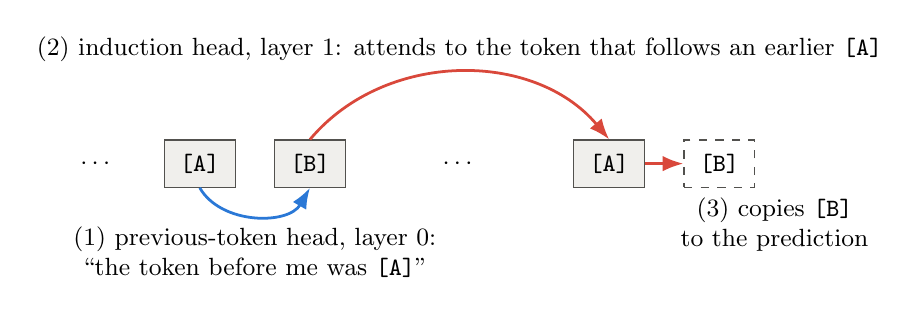
\begin{tikzpicture}[>=Latex, font=\small, tokn/.style={draw=tutgrey, fill=tutpaper, minimum height=6mm, minimum width=9mm}]
\node (l) at (0,0) {$\cdots$};
\node[tokn] (a1) at (1.3,0) {\tok{[A]}};
\node[tokn] (b1) at (2.7,0) {\tok{[B]}};
\node (m) at (4.6,0) {$\cdots$};
\node[tokn] (a2) at (6.5,0) {\tok{[A]}};
\node[tokn, dashed, fill=white] (b2) at (7.9,0) {\tok{[B]}};
\draw[->, line width=1pt, tutblue] (a1.south) to[out=-60,in=-120] node[below, text=black, align=center]
  {(1) previous-token head, layer 0:\\ ``the token before me was \tok{[A]}''} (b1.south);
\draw[->, line width=1pt, tutred] (b1.north) to[out=50,in=130] node[above, text=black, align=center]
  {(2) induction head, layer 1: attends to the token that follows an earlier \tok{[A]}} (a2.north);
\draw[->, line width=1pt, tutred] (a2.east) -- node[below=3mm, text=black, align=center, xshift=14mm] {(3) copies \tok{[B]}\\ to the prediction} (b2.west);
\end{tikzpicture}
\caption{The induction circuit. Arrows show the flow of information from a source position to a destination
position. The dashed box is the predicted next token.}
\label{fig:induction}
\end{figure}

Induction heads are not a curiosity of toy models. \citet{olsson2022context} found them in models of many
sizes and showed that they form during a short window early in training, at the same time as the model's
ability to use its context improves sharply. They are a mechanism of \emph{in-context learning}: the model picks
up a pattern from the prompt and continues it. Heads 5.5 and 6.9 of GPT-2 small are induction heads, and we have
already met them in \cref{tab:heads}.

\subsection{The IOI circuit}
\label{sec:ioi}

We can now assemble the evidence on the running example into the circuit of \citet{wang2023interpretability},
shown in \cref{fig:ioi}. As in their paper, we work backwards from the output.

\paragraph{Who writes the answer?} The name mover heads 9.9, 9.6 and 10.0. At the last position they attend to
the indirect object (\cref{sec:attention}) and write in the direction that raises its logit (\cref{fig:dla}).
Their $W_{OV}$ copies the name they attend to.

\paragraph{Why do they attend to the right name?} Both names are candidates. The name movers avoid the subject
because of the S-inhibition heads 7.3, 7.9, 8.6 and 8.10. These heads sit at the last position and attend to
S2. They write a signal into the last position that changes the queries of the name movers, so that positions
holding the subject receive less attention. This is the transfer from S2 to the last position in layers 7 and 8
that we saw in \cref{fig:residpatch}, and it explains why these heads have a large patching effect and a small
direct effect in \cref{tab:heads}.

\paragraph{How do the S-inhibition heads know which name is repeated?} Two groups of heads at S2 detect the
repetition. The duplicate token heads 0.1 and 3.0 attend from S2 to the earlier occurrence S1 of the same
token. The induction heads 5.5 and 6.9 attend from S2 to the token \emph{after} S1, using the output of the
previous-token heads 2.2 and 4.11 exactly as in \cref{sec:induction}. Both groups write to the stream at S2 that
this token has occurred before, and the S-inhibition heads read it.

\begin{figure}[t]
\centering
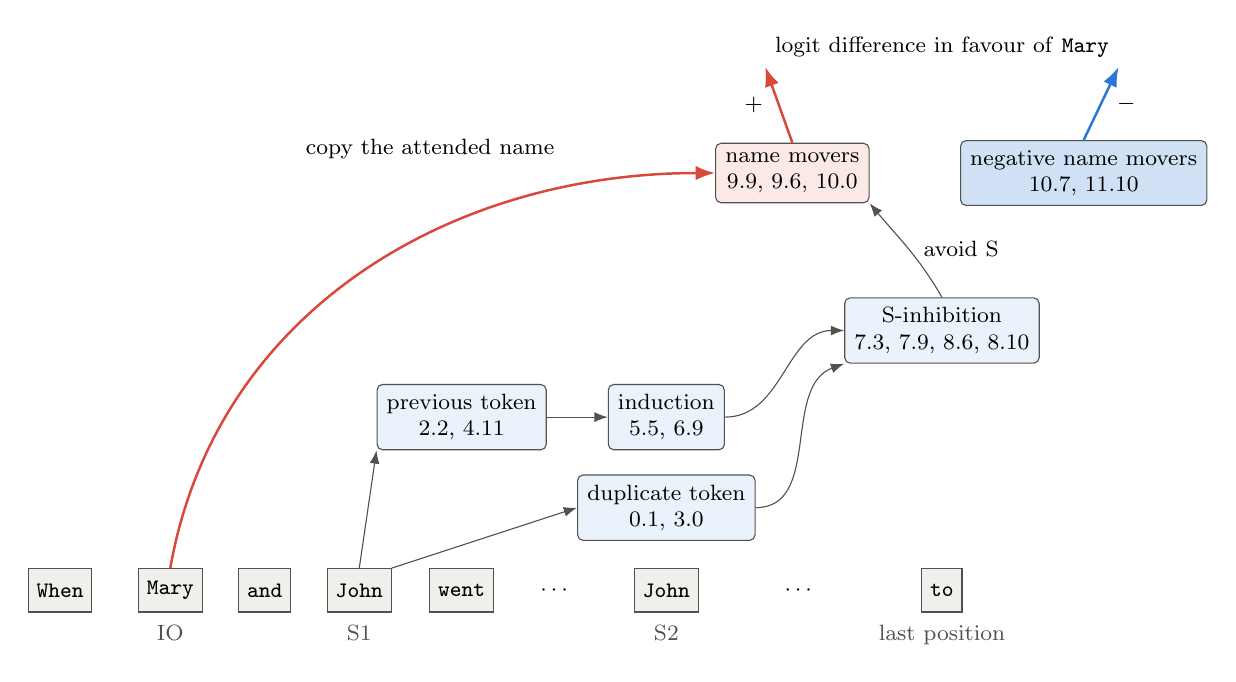
\begin{tikzpicture}[>=Latex, font=\footnotesize,
  tokn/.style={draw=tutgrey, fill=tutpaper, minimum height=5.5mm, inner sep=3pt},
  cls/.style={draw=tutgrey, rounded corners=2pt, align=center, inner sep=3.5pt, fill=#1}, cls/.default=tutblue!10]
\node[tokn] (t1) at (0,0) {\tok{When}};
\node[tokn] (io) at (1.4,0) {\tok{Mary}};
\node[tokn] (t3) at (2.6,0) {\tok{and}};
\node[tokn] (s1) at (3.8,0) {\tok{John}};
\node[tokn] (s1p) at (5.1,0) {\tok{went}};
\node (d1) at (6.3,0) {$\cdots$};
\node[tokn] (s2) at (7.7,0) {\tok{John}};
\node (d2) at (9.4,0) {$\cdots$};
\node[tokn] (end) at (11.2,0) {\tok{to}};
\node[below=1pt of io, tutgrey] {IO};
\node[below=1pt of s1, tutgrey] {S1};
\node[below=1pt of s2, tutgrey] {S2};
\node[below=1pt of end, tutgrey] {last position};
\node[cls] (prev) at (5.1,2.2) {previous token\\ 2.2, 4.11};
\node[cls] (dup) at (7.7,1.05) {duplicate token\\ 0.1, 3.0};
\node[cls] (ind) at (7.7,2.2) {induction\\ 5.5, 6.9};
\node[cls] (sinh) at (11.2,3.3) {S-inhibition\\ 7.3, 7.9, 8.6, 8.10};
\node[cls=tutred!12] (nm) at (9.3,5.3) {name movers\\ 9.9, 9.6, 10.0};
\node[cls=tutblue!22] (neg) at (13.0,5.3) {negative name movers\\ 10.7, 11.10};
\node (out) at (11.2,6.9) {logit difference in favour of \tok{Mary}};
\node at (4.7,5.6) {copy the attended name};
\draw[->, tutgrey] (s1.north) -- (prev.south west);
\draw[->, tutgrey] (s1.north east) -- (dup.west);
\draw[->, tutgrey] (prev.east) -- (ind.west);
\draw[->, tutgrey] (dup.east) to[out=0,in=200] (sinh.south west);
\draw[->, tutgrey] (ind.east) to[out=0,in=180] (sinh.west);
\draw[->, tutgrey] (sinh.north) to[out=120,in=-50] node[right=2pt, pos=0.5, text=black] {avoid S} (nm.south east);
\draw[->, tutred, line width=0.9pt] (io.north) to[out=80,in=180] (nm.west);
\draw[->, tutred, line width=0.9pt] (nm.north) -- node[left=2pt, text=black] {$+$} (out.south west);
\draw[->, tutblue, line width=0.9pt] (neg.north) -- node[right=2pt, text=black] {$-$} (out.south east);
\end{tikzpicture}
\caption{The circuit for indirect object identification in GPT-2 small, simplified from
\citet{wang2023interpretability}. Each box is a class of attention heads, drawn above the position at which the
heads write. Arrows show the flow of information. The backup name movers are omitted.}
\label{fig:ioi}
\end{figure}

\paragraph{The algorithm.} In words, the model does three things. It finds the name that occurs twice. It
tells the last position to ignore that name. It copies the name that is left. Two further classes complicate
the picture. The negative name movers 10.7 and 11.10 attend to the same name as the name movers and write
\emph{against} it, and the backup name movers become active when the name movers are removed. We saw the trace
of both in \cref{fig:lens,tab:heads}.

\paragraph{How good is the explanation?} The circuit of \citet{wang2023interpretability} has 26 heads in seven
classes (the count in the arXiv version of the paper and in the released code). On their distribution of
prompts the full model has an average logit difference of $3.56$. With every head outside the circuit
mean-ablated, the difference between circuit and full model is $13\%$ of that value, so the circuit retains
$87\%$. This is a strong result, and it also marks the limits of the best-understood circuit in a real language
model. It concerns one narrow task on templated prompts. A part of the behaviour remains unexplained. Several
classes of heads (negative and backup name movers) are described without a clear account of why training
produced them. And the role of the MLPs is left open.

\begin{caution}
Our own figures on 12 prompts reproduce the observational and single-node signatures of this circuit. They are
not a validation of it. We did not run path patching, and we did not test faithfulness, completeness or
minimality.
\end{caution}

\subsection{A network that was understood completely}
\label{sec:modadd}

For one family of small networks the reverse engineering has been carried to the end.
\citet{nanda2023progress} trained a one-layer transformer to add two numbers modulo $P=113$. The input is the
sequence $a$, $b$, \tok{=} with $a,b\in\{0,\dots,P-1\}$, and the correct output is the number
$c\in\{0,\dots,P-1\}$ with $c\equiv a+b \pmod P$. The network was trained on $30\%$ of all pairs. It first
memorises these and much later, quite suddenly, becomes correct on the rest. This delayed generalisation is
called \emph{grokking} \citep{power2022grokking}.

One would expect the network to learn something like a look-up table. It does something else. It uses a small
set of integer frequencies $r$ (five in the main model of the paper) and proceeds as follows.
\begin{enumerate}
\item The embedding maps the input $a$ to the numbers $\cos(2\pi ra/P)$ and $\sin(2\pi ra/P)$ for each of these
frequencies, and likewise for $b$.
\item Attention and MLP multiply these numbers and combine the products, by the addition theorems, into the
cosine and sine of the sum. For the cosine,
\[
\cos\!\Big(\frac{2\pi r(a+b)}{P}\Big)=\cos\!\Big(\frac{2\pi ra}{P}\Big)\cos\!\Big(\frac{2\pi rb}{P}\Big)
-\sin\!\Big(\frac{2\pi ra}{P}\Big)\sin\!\Big(\frac{2\pi rb}{P}\Big).
\]
\item The unembedding multiplies these with $\cos(2\pi rc/P)$ and $\sin(2\pi rc/P)$ for every candidate $c$.
By the addition theorem once more,
\[
\cos\!\Big(\frac{2\pi r(a+b)}{P}\Big)\cos\!\Big(\frac{2\pi rc}{P}\Big)
+\sin\!\Big(\frac{2\pi r(a+b)}{P}\Big)\sin\!\Big(\frac{2\pi rc}{P}\Big)
=\cos\!\Big(\frac{2\pi r(a+b-c)}{P}\Big).
\]
The logit of $c$ is approximately proportional to the sum of these terms over the frequencies,
\begin{equation}\label{eq:modadd}
\sum_{r}\cos\!\Big(\frac{2\pi r\,(a+b-c)}{P}\Big).
\end{equation}
\end{enumerate}

Why does \eqref{eq:modadd} single out the correct answer? If $c\equiv a+b$, every cosine equals $1$. For any
other $c$ the cosines of different frequencies point in different directions and largely cancel. With all
frequencies the cancellation is exact.

\begin{proposition}[Cosines over all frequencies form an indicator]\label{prop:cos}
Let $P\ge2$ be an integer and let $q$ be an integer. Then
\[
\sum_{r=0}^{P-1}\cos\!\Big(\frac{2\pi rq}{P}\Big)=\begin{cases}P&\text{if $q$ is divisible by $P$,}\\ 0&\text{otherwise.}\end{cases}
\]
\end{proposition}
\begin{proof}
If $q$ is divisible by $P$, every angle $2\pi rq/P$ is a multiple of $2\pi$, every term is $1$ and the sum is
$P$. Now let $q$ not be divisible by $P$. Then $\pi q/P$ is not a multiple of $\pi$, so $\sin(\pi q/P)\ne0$.
We multiply the sum by $2\sin(\pi q/P)$ and use the identity $2\sin\phi\cos\psi=\sin(\psi+\phi)-\sin(\psi-\phi)$
with $\phi=\pi q/P$ and $\psi=2\pi rq/P$.
\begin{align*}
2\sin\!\Big(\frac{\pi q}{P}\Big)\sum_{r=0}^{P-1}\cos\!\Big(\frac{2\pi rq}{P}\Big)
&= \sum_{r=0}^{P-1}\Big[\sin\!\Big(\frac{(2r+1)\pi q}{P}\Big)-\sin\!\Big(\frac{(2r-1)\pi q}{P}\Big)\Big] && \by{by the identity}\\
&= \sin\!\Big(\frac{(2P-1)\pi q}{P}\Big)-\sin\!\Big(\frac{-\pi q}{P}\Big) && \by{telescoping sum}\\
&= \sin\!\Big(2\pi q-\frac{\pi q}{P}\Big)+\sin\!\Big(\frac{\pi q}{P}\Big) && \by{since $\sin$ is odd}\\
&= -\sin\!\Big(\frac{\pi q}{P}\Big)+\sin\!\Big(\frac{\pi q}{P}\Big) \;=\; 0. && \by{period $2\pi$, $q$ an integer}
\end{align*}
Dividing by $2\sin(\pi q/P)\ne0$ gives the claim.
\end{proof}

With $q=a+b-c$, the proposition says that the sum \eqref{eq:modadd} over \emph{all} frequencies is $P$ for the
correct $c$ and $0$ for every other $c$. The trained network uses only five frequencies, and this is enough.
Since $P$ is prime, $\cos(2\pi rq/P)=1$ with $0<r<P$ forces $q$ to be divisible by $P$. So the sum of five
cosines equals $5$ at the correct answer and is strictly smaller everywhere else. \Cref{fig:modadd} shows how
large the margin is.

\begin{figure}[t]
\centering
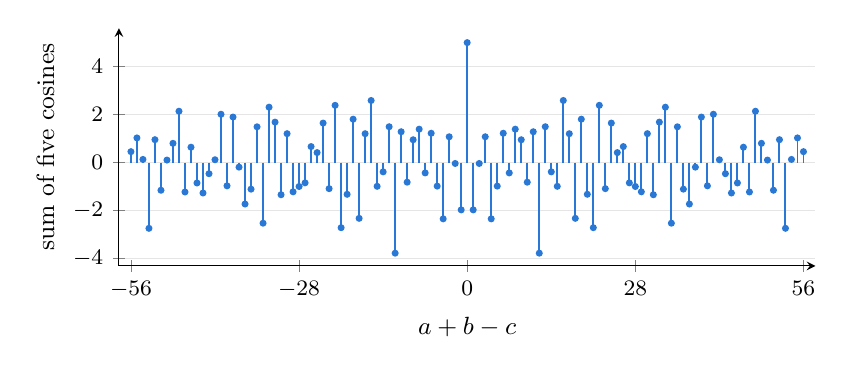
\begin{tikzpicture}
\begin{axis}[width=0.86\textwidth, height=4.6cm, xmin=-58, xmax=58, ymin=-4.3, ymax=5.6, axis lines=left,
  xlabel={$a+b-c$}, ylabel={sum of five cosines}, label style={font=\small}, tick label style={font=\footnotesize},
  xtick={-56,-28,0,28,56}, ytick={-4,-2,0,2,4}, ymajorgrids, grid style={black!10}]
\addplot[ycomb, tutblue, line width=0.7pt, mark=*, mark size=0.9pt, samples at={-56,...,56}]
  {cos(360*14*x/113)+cos(360*35*x/113)+cos(360*41*x/113)+cos(360*42*x/113)+cos(360*52*x/113)};
\end{axis}
\end{tikzpicture}
\caption{The sum \eqref{eq:modadd} for $P=113$ and the five frequencies $r\in\{14,35,41,42,52\}$ reported by
\citet{nanda2023progress}, as a function of $a+b-c$. The value is $5$ at the correct answer $a+b-c=0$ and at
most $2.59$ at every other residue.}
\label{fig:modadd}
\end{figure}

The authors did not guess this algorithm. They found periodic structure in the embedding matrix, traced it
through the network and confirmed each step by interventions. Removing the key frequencies destroys the
performance, and removing everything else improves it. They report that \eqref{eq:modadd} accounts for $95\%$ of
the variance of the logits.

Understanding the mechanism paid off in a second way. Knowing which weights belong to the trigonometric
algorithm, the authors could measure its strength during training. The algorithm does not appear at the moment
when the test loss falls. It is built up gradually while the network still relies on memorisation, and the
sudden improvement happens when weight decay finally removes the memorised solution. The three phases are
called memorisation, circuit formation and cleanup. A curve that looks like a sudden jump from the outside is a
gradual process on the inside.

\subsection{Scaling up: automatic discovery and feature circuits}
\label{sec:featurecircuits}

The IOI circuit took months of manual work on one task in a small model. Two lines of research try to scale
the approach.

\paragraph{Automatic search.} ACDC \citep{conmy2023towards} starts from the full graph and visits its edges
from the output towards the input. An edge is removed if patching it changes the output distribution by less
than a threshold. What remains is the circuit. Edge attribution patching \citep{syed2024attribution} replaces
the exact patching by the linear estimate of \cref{sec:attrpatching}, which makes the search fast. The
numbers that such methods report depend on the kind of ablation and on other details of the procedure
\citep{miller2024transformer}, and should be compared only under identical settings.

\paragraph{Better units.} Heads and neurons are the units that the architecture provides. As
\cref{sec:features} explained, they are mixtures of many features. \emph{Feature circuits} use SAE latents as
nodes \citep{marks2025sparse}. The most developed form is the \emph{attribution graph} of
\citet{ameisen2025circuit}. Its construction has four steps.
\begin{enumerate}
\item All MLPs are replaced by transcoders (\cref{sec:transcoders}), in a variant that lets a latent write to
several later layers. \citet{lindsey2025biology} use 30 million latents for the model Claude 3.5 Haiku.
\item The analysis is done for one prompt. The attention patterns and the scales in $\LN$ are frozen at the
values they take on this prompt.
\item At every layer and position an \emph{error node} is added, equal to the difference between the true MLP
output and the transcoder output. The resulting \emph{local replacement model} then reproduces the activations
of the real model on this prompt exactly.
\item In the local replacement model, every latent influences every later latent through linear maps only. The
direct effect of one latent on another is given by a formula, and the latents and effects that matter for the
output form the attribution graph.
\end{enumerate}
The graph is a hypothesis about the real model. It is tested by interventions in the real model: one suppresses
or activates a latent and checks that the output changes as the graph predicts.

Two findings of \citet{lindsey2025biology} show what such graphs can reveal. For the prompt asking for the
capital of the state that contains Dallas, the graph contains latents for Texas between the input and the answer
\tok{Austin}: the model performs the two steps internally. When writing rhyming verse, the model activates
candidate rhyme words at the end of a line \emph{before} it writes the next line, and then composes the line
so that it ends in one of them. The model plans ahead.

\begin{caution}
An attribution graph describes one prompt. It takes the attention patterns as given, so it does not explain
why the model attends where it does. The error nodes can carry a substantial share of the effect, and that
share is unexplained by construction. And the latents inherit every limitation of \cref{sec:sae}. The honest
summary of a graph is ``this is a mechanism consistent with the model's computation on this prompt, as far as
the replacement captures it''.
\end{caution}

\begin{takeaways}
A circuit is a subgraph of components with a description of what each one computes, and it has to be tested
for faithfulness, completeness and minimality. In small models circuits can be read from the weights. The
induction circuit and the IOI circuit show how heads compose into algorithms, and the modular addition network
shows that a learned algorithm can be understood completely and can differ from anything a programmer would
write. Attribution graphs extend the approach to large models, one prompt at a time and with an unexplained
remainder.
\end{takeaways}

\begin{exercise}\label{ex:skiptrigram}
In the model \eqref{eq:onelayer} with a single head, suppose the head makes ``\tok{keep} $\dots$ \tok{in}
$\to$ \tok{mind}'' and ``\tok{keep} $\dots$ \tok{at} $\to$ \tok{bay}'' likely. Using the three tables of
\cref{sec:pathexp}, argue that it will also raise the probability of ``\tok{keep} $\dots$ \tok{in} $\to$
\tok{bay}'' to some extent. Which table would have to depend on the destination token to avoid this?
\end{exercise}
\begin{exercise}\label{ex:induction}
Explain why the induction circuit of \cref{sec:induction} cannot be implemented by a transformer with one
layer. Use the fact that in \eqref{eq:path} the attention score depends only on the tokens $t_i$ and $t_j$ and
their positions.
\end{exercise}
\begin{exercise}\label{ex:cosprime}
Let $P=113$ and $r=14$. For which integers $q$ is $\cos(2\pi rq/P)=1$? Why does the argument fail for $P=112$?
\end{exercise}

\section{How not to fool yourself}
\label{sec:pitfalls}

Interpretability has no ground truth. Nobody can open a language model and look up the right answer, so an
explanation can only be checked against its own predictions. The history of the field contains many results
that looked convincing and turned out to be artefacts. This section collects the main ways in which that
happens, each with the control experiment that guards against it. Most of them have already appeared in the
Caution boxes.

\subsection{Eight failure modes}

\paragraph{1. Decodable is not used.} A probe or a latent shows that information is present. It does not show
that the model reads it (\cref{sec:probing}). \emph{Control:} intervene on the representation and check that the
behaviour changes as predicted.

\paragraph{2. The method explains the data and not the model.} Some saliency maps survive the replacement of
the weights by random numbers \citep{adebayo2018sanity}, and SAEs find readable latents in randomly initialised
transformers \citep{heap2025sparse}. \emph{Control:} run the identical pipeline on a model with random weights
and on shuffled labels. Whatever survives is not about what the model has learned.

\paragraph{3. The strongest examples flatter.} The top activations of a neuron or latent can suggest a clean
concept that fails on the bulk of its activations and on other data sets
\citep{bolukbasi2021interpretability}. \emph{Control:} sample examples from the whole range of activations, use
a second corpus, and measure how often the concept occurs \emph{without} the unit firing.

\paragraph{4. The intervention leaves the training distribution.} Zero ablation and strong steering produce
activations that the model has never seen. The resulting behaviour may reflect the damage and not the role of
the component (\cref{sec:interventions}). \emph{Control:} prefer replacement values that occur naturally, report
the size of the intervention relative to typical activations, and check that unrelated outputs stay intact.

\paragraph{5. Compensation hides importance.} In \cref{tab:heads}, corrupting the most important head changed
the output by a fifth of its direct effect, because later layers made up for it. \emph{Control:} report direct
and total effects, and ablate groups of components that may substitute for one another.

\paragraph{6. A successful intervention through the wrong pathway.} A direction or subspace found by
optimisation can produce the predicted behaviour by activating something the model does not normally use
\citep{makelov2024subspace}. \emph{Control:} verify that the direction varies in normal operation in the way the
hypothesis says, and that the effect disappears along directions chosen at random or orthogonally.

\paragraph{7. Localising is not understanding.} \citet{meng2022locating} located factual associations in the
MLPs of middle layers by patching, and edited the facts by changing weights there. \citet{hase2023does} then
found that the layer indicated by patching does not predict which layer is best to edit. Knowing where an
intervention has an effect, and knowing how the computation works, are different things. \emph{Control:} do not
use the success of an edit as evidence for a mechanism, or the reverse.

\paragraph{8. A narrow distribution and a good story.} The IOI circuit was established on templated
sentences, and an attribution graph on one prompt. Labels such as ``name mover'' are summaries made by people,
and a label can be more general or more specific than what the component does. \emph{Control:} state the
distribution on which the claim was tested, derive a prediction for inputs outside it, test that prediction,
and report the share of the behaviour that the explanation leaves open.

\begin{exercise}[\extitle{Base rates}{derivation}]\label{ex:baserate}
A latent fires on $90\%$ of the texts about a certain concept and on $5\%$ of all other texts. The concept occurs
in $1\%$ of the corpus. (a) Which fraction of the texts on which the latent fires is about the concept?
(b) Suppose that the latent fires more strongly on texts about the concept than on other texts. What will the
list of its $20$ strongest activations look like, and what will a reader of that list conclude? (c) Which control
of failure mode 3 reveals the problem?
\end{exercise}

\subsection{Matching the evidence to the claim}

A useful habit is to ask of every claim, including one's own, which kind of evidence it would need.
\Cref{tab:evidence} gives the minimum for the four kinds of claims that occur most often.

\begin{table}[t]
\centering\small
\begin{tabular}{@{}p{0.34\textwidth}p{0.6\textwidth}@{}}
\toprule
Claim & Minimal evidence \\
\midrule
``Property $y$ is represented in activation $x$.'' & A probe or latent with held-out accuracy, a control task or
shuffled labels, and the same analysis on a model with random weights. \\ \addlinespace
``The model uses this representation.'' & An intervention on the representation that changes the behaviour as
predicted, with a random direction of equal size as comparison. \\ \addlinespace
``Component $g$ matters for task $T$.'' & Patching or ablation with a stated replacement value and a stated
distribution of prompts. Direct and total effect. \\ \addlinespace
``This circuit is how the model does $T$.'' & Faithfulness, completeness and minimality. A confirmed prediction
on new inputs. The size of the unexplained remainder. \\
\bottomrule
\end{tabular}
\caption{The weakest evidence that supports each common type of claim. A weaker kind of evidence supports only
a weaker claim.}
\label{tab:evidence}
\end{table}

\begin{exercise}[\extitle{A lie detector}{concept}]\label{ex:critique}
A blog post reports: ``We trained a linear probe on layer 20 of a chat model and can predict with 99\% accuracy
whether the model is about to lie. We have found the model's lie detector.'' List three experiments that are
missing, and say for each which failure mode of this section it addresses.
\end{exercise}

\begin{exercise}[\extitle{Three abstracts}{concept}]\label{ex:abstracts}
For each of the following summaries, name the row of \cref{tab:evidence} to which the claim belongs and the most
important piece of evidence that is missing. (a) ``Zero-ablating the MLP of layer 14 destroys the ability of the
model to add two-digit numbers. Addition is therefore computed in this MLP.'' (b) ``A latent of our SAE fires on
$85\%$ of the answers in which the model deceives the user. The model therefore knows when it is deceiving.''
(c) ``Our automatically discovered circuit reaches $98\%$ faithfulness under mean ablation. It contains $70\%$ of
all edges of the model.''
\end{exercise}

\begin{exercise}[\extitle{A baseline for steering}{concept}]\label{ex:steerbaseline}
Adding a steering vector raises the rate of a certain behaviour from $10\%$ to $60\%$. Adding a random vector of
the same norm raises it to $35\%$. (a) Which part of the increase can be credited to the direction? (b) Suggest a
reason why a random vector changes the behaviour at all. (c) Which further measurements are needed before the
vector is used to control the model?
\end{exercise}

\begin{takeaways}
Before believing an interpretability result, ask six questions. What exactly is the hypothesis, and what would
count against it? On which distribution of inputs was it tested? What was the counterfactual in each
intervention? Does the result disappear for a random model, random labels or a random direction? Is the
evidence observational or interventional, and does the claim go beyond it? How much of the behaviour is left
unexplained?
\end{takeaways}

\begin{readinglist}
\item \citet{adebayo2018sanity}, \emph{NeurIPS}, and \citet{heap2025sparse}, \emph{ICLR}. The same control, a model
with random weights, applied to attribution maps and to sparse autoencoders (failure mode 2).
\item \citet{hewitt2019designing}, \emph{EMNLP}. Control tasks, the standard guard against failure mode 1.
\item \citet{makelov2024subspace}, \emph{ICLR}. A complete worked example of failure mode 6, on the IOI task.
\item \citet{hase2023does}, \emph{NeurIPS}. The evidence behind failure mode 7.
\item \citet{friedman2024interpretability}, \emph{ICML}. Simplified descriptions of a model can agree with it on
the training distribution and disagree elsewhere (failure mode 8).
\item \citet{miller2024transformer}, \emph{COLM}. Shows how much reported faithfulness depends on details of the
ablation.
\item \citet{shi2024hypothesis}, \emph{NeurIPS}. Turns the criteria for circuits into statistical hypothesis
tests and applies them to published circuits.
\item \citet{meloux2025everything}, \emph{ICLR}. Enumerates all candidate explanations in small networks and finds
that many different ones pass the usual criteria. An explanation that passes need not be the only one.
\end{readinglist}

\section{Where to go from here}
\label{sec:practice}

\subsection{Software and a first experiment}

Everything in this tutorial can be reproduced on a laptop. The standard open-source tools are the following.

\begin{itemize}
\item \textbf{TransformerLens} \citep{nanda2022transformerlens} loads open models and gives access to every
intermediate activation through named \emph{hooks}. It is the usual choice for small models.
\item \textbf{nnsight} \citep{fiottokaufman2025nnsight} offers the same kind of access for arbitrary PyTorch
models, including large ones that run on a remote server.
\item \textbf{SAELens} \citep{bloom2024saelens} trains sparse autoencoders and loads published ones, such as
Gemma Scope \citep{lieberum2024gemma}.
\item \textbf{Neuronpedia} \citep{lin2023neuronpedia} is a website on which the latents of published
dictionaries can be browsed, tested on one's own text and used for steering. It also hosts attribution graphs.
\end{itemize}

The listing below is the complete code for the patching experiment of \cref{fig:residpatch} on a single pair of
prompts. It prints a logit difference of $3.36$ for the clean prompt and $-2.48$ for the corrupted one, and
then the effect at S2 and at the last position for each layer. The script \texttt{code/gpt2\_examples.py}
extends it to all figures of this tutorial.

\lstinputlisting[style=tutpython]{code/minimal_patching.py}

\begin{caution}
The listing was tested with TransformerLens 4.4. Older tutorials use the class \texttt{HookedTransformer},
which was removed in version 4.0 in September 2026. They run unchanged with an older version of the
library (\texttt{pip install "transformer-lens<4"}). The names of the hooks are the same in both.
\end{caution}

\subsection{Five first projects}

Reading about interpretability teaches less than doing it. The following projects are ordered by difficulty,
and each takes between an afternoon and a week.

\begin{enumerate}
\item \textbf{Break the running example.} Run the accompanying script. Then change the template: other verbs,
three names, the order of the clauses. Find out which of the figures of this tutorial change and which stay.
This is failure mode 8 of \cref{sec:pitfalls} in practice.
\item \textbf{Find the induction heads.} Feed GPT-2 small a sequence of random tokens followed by the same
sequence again. For every head, average the attention weight from each token of the second half to the token
after its first occurrence. A few heads will stand out. Compare them with \cref{tab:heads}.
\item \textbf{Solve the toy model.} Train the model \eqref{eq:toy} with $N=2$, $d=1$ for several values of
$\delta$ and compare the solution and its loss with \cref{prop:toy}. Then take $N=5$, $d=2$ and look for the
pentagon of \cref{fig:superposition}.
\item \textbf{Test a latent.} Pick a latent of a published dictionary on Neuronpedia. Write down a prediction
of where it fires and what it does when it is amplified. Then test both, including on text where it should
\emph{not} fire.
\item \textbf{Steer with controls.} Compute a difference of means \eqref{eq:diffmeans} for a simple contrast,
for example positive against negative reviews. Add it to the stream and measure the effect. Repeat with a random
direction of the same norm and with the direction found at another layer.
\end{enumerate}

\subsection{Open problems}

The field is young, and its foundations are still moving. Four questions are widely seen as open. The surveys
of \citet{sharkey2025open} and \citet{barez2026understanding} treat them at length.

\begin{itemize}
\item \textbf{What are the right units?} SAE latents are not canonical (\cref{sec:sae}). One alternative
decomposes the \emph{weights} of a network into simple parts instead of its activations
\citep{braun2025interpretability,bushnaq2025stochastic}. Another trains networks whose weights are sparse from
the start, which makes their circuits small and readable at some cost in capability \citep{gao2025weight}.
\item \textbf{How can an explanation be validated?} The tests of \cref{sec:circuits} work on narrow tasks. There
is no agreed standard for explanations of open-ended behaviour.
\item \textbf{What is the theory?} Why linear representations emerge, how much computation fits into
superposition, and when sparse dictionaries recover the true features are mathematical questions with partial
answers at best \citep{park2024linear,hanni2024mathematical,adler2024complexity}.
\item \textbf{What is it good for?} There is an active debate between two aims: the complete reverse engineering
of a network, and methods that are judged by their measurable use in tasks such as monitoring and auditing
\citep{nanda2025pragmatic,marks2025auditing}.
\end{itemize}

\subsection{What to read next}

\begin{itemize}
\item \citet{elhage2021mathematical} is the source of the residual-stream view of \cref{sec:transformer} and of
\cref{sec:pathexp}. Read it first.
\item \citet{elhage2022toy} develops superposition (\cref{sec:features}) with many experiments.
\item \citet{wang2023interpretability} is the model of a circuit analysis, and \citet{nanda2023progress} of a
complete one.
\item \citet{heimersheim2024use} is a practical guide to activation patching and its interpretation.
\item \citet{bricken2023monosemanticity} and \citet{templeton2024scaling} introduce sparse autoencoders, and
\citet{ameisen2025circuit} and \citet{lindsey2025biology} the attribution graphs built on them.
\item \citet{ferrando2024primer} and \citet{bereska2024mechanistic} are broad surveys. The glossary of
\citet{nanda2022glossary} explains the jargon of the field, and the ARENA course \citep{mcdougall2023arena}
teaches the methods through programming exercises.
\end{itemize}


\appendix
\section{Glossary}
\label{app:glossary}

{\footnotesize \setlength{\columnsep}{20pt}
\begin{multicols}{2}
\begin{description}[style=sameline, leftmargin=0pt, itemsep=1.5pt, font=\normalfont\bfseries]
\item[Ablation.] Replacing the value of a node by zero, by its mean or by its value on another prompt, and
measuring the change of the output (\cref{sec:interventions}).
\item[Activation.] Any intermediate value that the model computes on a given input.
\item[Activation patching.] Running the model on one prompt while overwriting one node with its value from a
second, minimally different prompt (\cref{sec:patching}).
\item[Attention head.] The component that moves information between positions. It is described by the matrices
$W_{QK}$ (from where to read) and $W_{OV}$ (what to write), see \eqref{eq:qkov}.
\item[Attention pattern.] The weights $A^{\ell,h}_{ij}$ with which head $h$ of layer $\ell$ at destination $i$
reads from the sources $j\le i$.
\item[Attribution graph.] A graph of transcoder latents and their direct effects on one another for a single
prompt (\cref{sec:featurecircuits}).
\item[Attribution patching.] The first-order estimate \eqref{eq:attrpatch} of the effect of activation patching.
\item[Circuit.] A subgraph of the model's components together with a description of what each one computes on
a task (\cref{def:circuit}).
\item[Clean and corrupted prompt.] The two prompts of a patching experiment. They differ only in the aspect
under study.
\item[Composition.] The use of the output of an earlier head in the query, key or value of a later head.
\item[Dictionary direction.] A column $\Wdec[j]$ of the decoder of a sparse autoencoder.
\item[Direct logit attribution.] The term that one component contributes to a logit through its own addition
to the residual stream (\cref{prop:dla}).
\item[Faithful.] Said of an explanation that correctly describes what the model computes. Opposed to merely
plausible.
\item[Feature.] A property of the input or of the intermediate computation that the model represents.
\item[Hook.] A place in the code of a model at which an activation can be read or overwritten.
\item[Latent.] One unit of a sparse autoencoder or transcoder. A candidate for a feature.
\item[Linear probe.] A logistic regression that predicts a label from an activation (\cref{sec:probing}).
\item[Logit.] The score of a token before the softmax \eqref{eq:softmax}.
\item[Logit difference.] The logit of the correct token minus that of a chosen alternative. Our metric
\eqref{eq:ld}.
\item[Logit lens.] Applying the final read-out to an intermediate residual stream \eqref{eq:lens}.
\item[Neuron.] One coordinate of the hidden layer of an MLP.
\item[Polysemantic.] Said of a neuron that responds to several unrelated features.
\item[Privileged basis.] A coordinate system that the architecture singles out, as the neurons of an MLP. The
residual stream has none.
\item[Residual stream.] The vector $x_i^{(\ell)}$ that is kept for each position and to which all components
add their output.
\item[Sparse autoencoder.] A wide one-layer autoencoder trained to reconstruct activations with few active
latents (\cref{sec:sae}).
\item[Steering.] Adding a direction to the residual stream, or removing it, to change a behaviour
(\cref{sec:steering}).
\item[Superposition.] The storage of more features than dimensions along almost orthogonal directions
(\cref{sec:superposition}).
\item[Token.] A word or word fragment. The unit in which the model reads and writes text.
\item[Transcoder.] A sparse, wide replacement of an MLP that predicts its output from its input.
\item[Unembedding.] The matrix $W_U$ that turns the final residual stream into logits.
\end{description}
\end{multicols}
}

\section{Solutions to the exercises}
\label{app:solutions}

{\small
\paragraph{\Cref{ex:params}.} A head has $4\cdot d\cdot d_{\mathrm{head}}=4\cdot768\cdot64=196{,}608$ weights. $W_E$ has
$50257\cdot768=38{,}597{,}376$ entries, which is $31\%$ of the model.

\paragraph{\Cref{ex:ones}.} Since $\mean(x+s\,\one)=\mean(x)+s$, we get
$x+s\,\one-\mean(x+s\,\one)\,\one=x-\mean(x)\,\one$. The numerator and the scale in \eqref{eq:ln} are therefore
unchanged. Every component reads the stream through $\LN$, so all component outputs stay the same. By
\eqref{eq:update}, all later streams at this position differ from the original ones by the same $s\,\one$, which
the final $\LN$ in \eqref{eq:unembed} removes.

\paragraph{\Cref{ex:rank}.} $W_{OV}=W_OW_V$ factors through $\R^{d_{\mathrm{head}}}$, so its rank is at most
$d_{\mathrm{head}}=64$. Whatever a head writes lies in the column space of $W_O$, a fixed subspace of dimension at
most $64$ of $\R^{768}$.

\paragraph{\Cref{ex:linearig}.} The gradient $\nabla_{z_i}F=w_i$ is constant, so
$\mathrm{IG}_i(z)=z_i^\top\int_0^1w_i\,du=w_i^\top z_i$, which is gradient times input. For $F(z)=z^2$ we have
$F'(z)=2z$. Gradient times input is $2z^2$, and $\mathrm{IG}(z)=z\int_0^12uz\,du=z^2=F(z)-F(0)$.

\paragraph{\Cref{ex:lenslast}.} At $\ell=L$, \eqref{eq:lens} is \eqref{eq:unembed}. The components up to layer 8
add up to $x_n^{(9)}$ by the proof of \cref{prop:sum}. Their DLA terms therefore add up to
$(W_U[\mathrm{IO}]-W_U[\mathrm{S}])^\top(x_n^{(9)}-\mean(x_n^{(9)})\,\one)/\scale(x_n^{(L)})$. The lens divides the same
numerator by $\scale(x_n^{(9)})$. The two numbers differ by the factor $\scale(x_n^{(9)})/\scale(x_n^{(L)})$.

\paragraph{\Cref{ex:probecontrol}.} Being a first name is a function of the current token, and the token is
encoded in $x_i^{(0)}$ by \eqref{eq:embed}. Train the same probe on layer $0$, and on a control task that gives
each token type a random label. The probe on layer $0$ will succeed as well, so the result shows nothing
specific about layer 6.

\paragraph{\Cref{ex:triangle}.} $v_i^\top v_j=\cos120^\circ=-1/2$. If only feature $i$ is active, $x=f_iv_i$. Then
$\relu(v_i^\top x)=f_i$ and, for $j\ne i$, $\relu(v_j^\top x)=\relu(-f_i/2)=0$. If no feature is active, $x=0$.

\paragraph{\Cref{ex:bound}.} $N\le e^{10.24}\approx2.8\times10^4$ for $\varepsilon=0.1$ and
$N\le e^{40.96}\approx6\times10^{17}$ for $\varepsilon=0.2$. The condition $k\varepsilon<1/2$ allows $k\le4$ and
$k\le2$.

\paragraph{\Cref{ex:nobias}.} Now $\hat f_2=0$ and the loss is $\E f_2^2=\delta/3$, which exceeds $\delta^2/3$ for
every $\delta<1$. The bias lets the model output the mean of the feature it ignores. This lowers the error from
the second moment $\delta/3$ to the variance $\delta/3-\delta^2/4$.

\paragraph{\Cref{ex:normconstraint}.} Since $\relu(y/2)=\relu(y)/2$, the new activation is $f_j(x)/2$. Its product
with the doubled column is unchanged, and its penalty is halved. Without the constraint, training would let the
columns grow and the activations shrink towards zero, and the penalty would lose its meaning.

\paragraph{\Cref{ex:fvu}.} The optimal value is $f=\max(0,f^\star-0.2)$. The error is $f^\star$ for $f^\star<0.2$
and $0.2$ otherwise. Hence $\E\,(f^\star-f)^2=\int_0^{0.2}u^2\,du+0.8\cdot0.04=0.0027+0.032\approx0.035$.

\paragraph{\Cref{ex:ggb}.} Observations: weak and medium activations are also about the bridge, and the latent
fires on most mentions of the bridge in a new corpus. Intervention: amplifying the latent makes the model talk
about the bridge, and a random latent of equal strength does not.

\paragraph{\Cref{ex:andor}.} (a) Denoising gives $\max(1,0)=1$, effect $1$. Noising gives $\max(0,1)=1$, effect
$0$. Each node is sufficient and none is necessary. (b) Denoising gives $\min(1,0)=0$, effect $0$. Noising
gives $\min(0,1)=0$, effect $1$. Each node is necessary and none is sufficient.

\paragraph{\Cref{ex:affine}.} An affine function has the same gradient everywhere, and its increment between two
points equals this gradient times their difference. Example: the node $\LN(x_n^{(L)})$ with the logit difference
as metric, by \eqref{eq:ld}.

\paragraph{\Cref{ex:projection}.} The map is $x\mapsto(I-vv^\top)x$, which is linear.
$(I-vv^\top)^2=I-2vv^\top+v(v^\top v)v^\top=I-vv^\top$. And $w^\top(I-vv^\top)x=w^\top x-(w^\top v)(v^\top x)=w^\top x$
when $w^\top v=0$.

\paragraph{\Cref{ex:skiptrigram}.} Both \tok{in} and \tok{at} attend to \tok{keep}. What the head then writes
depends only on the source \tok{keep}, and it promotes both \tok{mind} and \tok{bay}. So \tok{bay} is also
promoted after \tok{in}. To avoid this, the table $W_U[t]^\top W_{OV}^{0,h}W_E[t_j]$ would have to depend on the
destination token.

\paragraph{\Cref{ex:induction}.} The induction head has to attend to the position $j$ whose \emph{previous} token
equals the current token. In one layer, the score of the pair $(i,j)$ depends on $t_i$, $t_j$ and the positions,
and not on $t_{j-1}$. An earlier layer must first write $t_{j-1}$ into position $j$.

\paragraph{\Cref{ex:cosprime}.} $\cos(2\pi\cdot14q/113)=1$ holds exactly when $113$ divides $14q$, which means
that $113$ divides $q$, since $113$ is prime. For $P=112$ the number $14q/112=q/8$ is an integer for $q=8$, so a
wrong answer would score as high as the correct one at this frequency.

\paragraph{\Cref{ex:critique}.} A control task or shuffled labels, and a check that lying and honest prompts do
not differ in topic or length (modes 1 and 2). An intervention along the probe direction that changes whether
the model lies, compared with a random direction (modes 1 and 6). A test on lies of a different kind than those
in the training set (mode 8).
}


{\footnotesize \setlength{\bibsep}{2.5pt plus 1pt}
\bibliographystyle{plainnat}
\bibliography{references}
}

\end{document}
